\documentclass[webpdf,contemporary,large]{oup-authoring-template}
\usepackage{color}
\usepackage{soul}
%\usepackage{ctex}
\usepackage{graphicx}
\usepackage{amsmath}
\usepackage{booktabs}
\usepackage{float}
%\usepackage{indentfirst}
\graphicspath{{assets/}}

\begin{document}

\journaltitle{Journal Title Here}
\DOI{DOI added during production}
\copyrightyear{2026}
\pubyear{2026}
\vol{XX}
\issue{x}
\access{Published: Date added during production}
\appnotes{Paper}

\firstpage{1}

\title[Ocean Temperature and Salinity Prediction]{Ocean Temperature and Salinity Prediction Based on Spatiotemporal Enhanced ConvLSTM and Linear-Nonlinear Hybrid Ensemble}

\author{Author Name}

\abstract{Temperature and salinity are critical physical parameters of the ocean with immense research significance. In recent years, deep learning methods have been applied to the inversion of ocean temperature and salinity fields. However, most models fail to correctly combine spatiotemporal dependencies or lack physical consistency when performing long-term sequence modeling and multivariate collaborative prediction. To this end, this study proposes a Stacking fusion framework based on improved Convolutional Long Short-Term Memory network (ConvLSTM) to achieve high-resolution and high-precision inversion of ocean temperature and salinity fields. The model fuses multi-source ocean data such as subsurface ocean temperature and salinity profiles, sea surface height anomalies, and sea surface wind fields at the data layer. Structurally, it uses ConvLSTM with an Encoder-Decoder architecture as the backbone and introduces an attention refinement mechanism and residual connections to globally calibrate the long-term dependencies between features and enhance feature reuse capabilities. Finally, the model uses ARIMA to model the linear and seasonal components of each grid point sequence, and uses XGBoost as a Stacking meta-learner to fuse the output results of ARIMA and ConvLSTM, further reducing the error accumulation of multi-step prediction.
Inversion results for the Western Pacific show that the proposed model significantly outperforms benchmark models such as CNN and standard ConvLSTM in both temperature and salinity prediction. Its RMSE is reduced to 0.0871°C and 0.1327 PSU, respectively, an improvement of 42.4\% and 71.9\% compared to CNN. In addition, this study introduces two derived variables, Potential Density and Spiciness, as physical consistency evaluation metrics, verifying the significant effect of the model in maintaining seawater physical properties, providing a more objective tool for real ocean prediction.}

\keywords{Ocean Temperature and Salinity Prediction, ConvLSTM, Spatiotemporal Deep Learning, Attention Mechanism, Physical Consistency, Multi-source Data Fusion}

\maketitle

\section{Introduction}

\subsection{Research Background}

In contemporary ocean research, ocean temperature and salinity are very important environmental parameters, which have significant meaning in sonar detection, fishery resources, climate regulation, etc., and have very wide application scenarios.
First, the speed of sound in seawater is jointly determined by temperature, salinity, and pressure. The uneven distribution of ocean temperature and salinity leads to changes in the profile structure and horizontal distribution characteristics of sound speed in seawater \cite{LiuYuLiangSanWeiHaiYangWenYanChangZhiNengYuBaoJiYingYongYanJiu2025}, which in turn affects the path of sound wave refraction, thereby affecting the loss and concealment during sound wave propagation, and ultimately affecting the propagation of sound waves. Relevant studies in recent years have shown that the invention of the layered modeling method of sound speed field based on improved BPNN and the sound speed field construction method combining WOA18 temperature and salinity model and LSTM has further demonstrated the powerful ability of ocean temperature and salinity fields to characterize underwater sound speed profiles and underwater sound transmission paths, providing new technical methods for modeling underwater acoustic environments \cite{WangZhaoYingJiYuGaiJinBPNNDeShengSuChangFenCengJianMo2024,TangAnJiYuShenDuXueXiLianHeWOA18WenYanMoXingGouJianShengSuChang2024}.
In addition, under the background of modern ocean warming, changes in temperature and salinity fields have become key factors affecting fishery resources and biodiversity by influencing species distribution, community structure, and physiological metabolism \cite{DongZhiGuoHaiYangNuanHuaBeiJingXiaHaiYangYuYeZiYuanJiQiShengWuXiangYingDeYanJiuJinZhan2024}, which has a direct and profound impact on fishery production, biodiversity protection, and ecosystem stability.
Finally, in terms of climate system regulation, underwater temperature and salinity fields also play a crucial role in climate change\cite{YangNingShengWoGuoHaiYangXinXingChanYeZhanLueGaiGuan2014}. The temperature and salinity field directly drives the global thermohaline circulation by influencing the density distribution of seawater, thereby regulating the transport of heat and salt, and further affecting the changes of the global climate system. Relevant studies show that the global ocean thermohaline transport has obvious seasonal changes, and its distribution and intensity will directly affect the energy balance of the climate system \cite{CuiWeiJiYuZaiFenXiShuJuDeQuanQiuHaiYangShuiTiHeReYanShuYunJiQiJiJieBianHua2023}.

\subsection{Problem Statement}

\subsubsection{Challenges of Sparse and Highly Dynamic Spatiotemporal Ocean Data}

In this study, an important problem faced is the scarcity of ocean environmental data. Conventional ocean databases such as ARGO drifting buoys and satellite remote sensing have a series of problems such as insufficient coverage and discontinuous observations. As shown in the ocean temperature data figure below, it can be clearly seen that there is a large amount of missing ocean temperature data in the offshore waters around the land. Therefore, innovative means are needed to expand and enhance the dataset.

\begin{figure}[H]
\centering
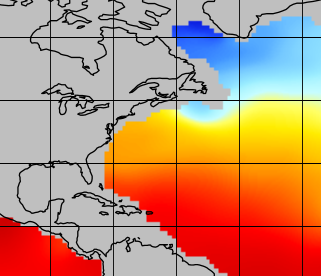
\includegraphics[width=\linewidth]{1765170582694-1.png}
\caption{Schematic of Missing Ocean Temperature Data}
\label{fig:temp_dist}
\end{figure}

\subsubsection{Limitations of Traditional Numerical Assimilation: High Computational Cost}

Traditional numerical assimilation methods have achieved relatively good results in improving forecast accuracy when conducting ocean research, but they also generally have the problem of excessive computational costs. For example, 4D-Var relies significantly on high-performance computing platforms, while EnKF needs to maintain a large number of ensemble members, and its task calculation amount and memory resource overhead increase with the growth of resolution and observation quantity. At the same time, since the construction of errors is not systematic, the assimilation system needs to be updated frequently to correct prediction results and reduce errors, thereby further increasing the computational burden. In summary, traditional assimilation methods are difficult to be widely applied in prediction scenarios with high resolution or strong real-time requirements.

\subsubsection{Current Status and Issues of Deep Learning Models in Ocean Forecasting}

In recent years, with the accumulation of computing power and massive ocean observation data, deep learning methods, led by Long Short-Term Memory networks, have been widely used in sea surface temperature and marine heatwave prediction tasks, showing prediction capabilities comparable to operational forecasting systems, especially having good prediction effects when the forecast lead time is short \cite{boninoMachineLearningMethods2024}. Compared with traditional numerical simulation and assimilation systems, such technologies can effectively capture the complex nonlinear relationships and spatiotemporal dependencies in ocean data \cite{zhaoDeepLearningOcean2024}.

However, the application process of deep learning in ocean prediction has not been smooth sailing. First, the training of many models relies heavily on training data, while ocean observation data often has problems such as sparsity and unevenness, making it difficult to cover all spatiotemporal ranges, which to some extent affects the training effect of the model and reduces the generalization ability of the model \cite{stortoCorrectionSeaSurface2025}. Second, for long-sequence multi-step prediction, deep models are prone to a series of problems such as blurring and loss of details. Especially when trying to predict nonlinear and fine-scale data, this blurring will weaken the credibility of the prediction results in a physical sense, thereby affecting the prediction effect. Third, various deep learning models such as ConvLSTM usually lack physical interpretability \cite{yangMultiFactorDeepLearning2025}. Various models rely solely on data driving, so their subjective and objective consistency with real physics is usually weak, which is unfavorable for scientific research and engineering application. Finally, most deep learning models are currently still good at predicting short-term or medium-term data changes. Many models ignore dynamic spatial dependencies and long-term temporal patterns such as seasonal cycles, which limits their ability to make accurate and stable long-term forecasts \cite{haoInterpretableCrossSphereMultiscale2025}.

\subsection{Contributions}

\subsubsection{Construction of a Multivariate Ocean Temperature-Salinity Inversion Framework Based on ConvLSTM}

Aiming at a series of related problems faced by current research on ocean temperature and salinity fields, this study successfully constructed a Convolutional Gated Recurrent Network for predicting 3D temperature and salinity field sequences. The model includes and combines spatial convolution and temporal recursion, thereby completing the spatiotemporal correlation of model prediction, rather than predicting time or space alone. In addition, this project also introduced an attention refinement module. By combining the model architecture with the attention mechanism, the model constructed in this study can more effectively capture the interactions between physical variables such as temperature, salinity, and ocean currents, thereby improving the sea surface temperature prediction ability for multiple forecast lead times \cite{yangMultiFactorDeepLearning2025}. In addition, the model achieves multivariate coupled output and multi-step prediction on the output capable of inverting and spatiotemporally predicting temperature and salinity at a certain point in the ocean.

\subsubsection{Addressing Insufficient Training Samples with Two Data Augmentation Methods}

Aiming at the problem of insufficient training samples, this study adopted two methods: spatial sliding window and equatorial symmetry filling for data augmentation. By innovatively combining the two methods to enhance and expand data samples, the sample size requirements for model training and prediction were met, achieving considerable experimental results.

\subsubsection{Physical Consistency Assessment}

In the process of model testing and comparative evaluation in the sixth part, this study not only used traditional error variables such as MAE, RMSE, and R-squared, but also derived and calculated several derived physical quantities related to ocean temperature and salinity data through relevant physical formulas of ocean temperature and salinity fields. This allows to further judge whether the prediction results follow objective and necessary physical relationships, making the final test conclusions not only statistically accurate and reliable, but also more objectively credible and persuasive in a physical sense.

\section{Related Work}

\subsection{Traditional Numerical Ocean Models}

Traditional ocean numerical models are mainly based on basic ocean dynamic equations such as continuity equations and conservation of heat and salt to numerically solve ocean circulation, temperature and salinity distribution, and energy transport. Representative models include HYCOM (Hybrid Coordinate Ocean Model) and ROMS (Regional Ocean Modeling System).
The HYCOM model framework adopts a hybrid vertical coordinate system, capable of adaptively switching between $\sigma$ coordinates, isopycnic coordinates, and z coordinates in different depth regions, thereby more accurately characterizing the density layer structure and large-scale ocean circulation features \cite{bleckOceanicGeneralCirculation2002}. ROMS is a three-dimensional ocean circulation model with a free surface, terrain-following coordinate system, and primitive control equations \cite{LiZhenXiTaiPingYangYangLiuXiTongDuiHaiPingMianGaoDuBianHuaDeXiangYingJiYuQuYuHaiYangMoShiROMSShiYan2025}.
In recent years, traditional physical ocean numerical models have been used to predict future ocean temperature fields. Based on physical equations and oceanographic principles, these models establish a series of equations to simulate ocean temperature distribution and provide relatively reliable temperature predictions according to initial condition.

\subsection{Deep Learning-Based Spatiotemporal Prediction}

\subsubsection{Applications of RNN and LSTM in Time Series Prediction}

Recurrent Neural Networks (RNN) and Long Short-Term Memory networks (LSTM) can effectively capture nonlinear spatiotemporal dependencies and are models often used by people when modeling time series. RNN can be used to process time series data, while LSTM, as a product of RNN development, effectively improved RNN and can cope with different types of time series data training \cite{SunMiaoShenDuXueXiZaiHaiYangDaShuJuWaJueZhongDeYingYong2018}. Through the gating mechanism, LSTM can selectively retain and update historical information, which can effectively alleviate the gradient vanishing problem generated under long-term dependencies \cite{YangJunGangJiYuYaoGanDeHaiYangSanWeiWenYanChangZhiNengTanCeYanJiuJinZhan2024}, so it is widely used in time series prediction and multivariate time series modeling in the ocean field. In relevant studies conducted so far, the encoder-decoder structure based on LSTM has shown high prediction accuracy and good stability when conducting short-term forecasting for seawater temperature profiles in a certain area of the South China Sea, verifying the effectiveness of LSTM in ocean environmental parameter prediction \cite{FanPeiQinJiYuLSTMWangLuoDeHaiShuiWenDuPouMianYuBaoYanJiu2024}. However, it should be noted that the LSTM model itself is mainly modeled for the time dimension. When directly used for high-dimensional grid fields, without appropriate spatial encoding, it will lose neighborhood spatial structure information. Therefore, it is often used in combination with convolutional structures or spatial attention modules in spatial field prediction tasks to simultaneously preserve temporal and spatial features.

\subsubsection{Applications of ConvLSTM and Its Variants (PredRNN, SA-ConvLSTM) in SST Prediction}

ConvLSTM (Convolutional Long Short-Term Memory Network) ingeniously combines Convolutional Neural Networks (CNNs) and Long Short-Term Memory networks (LSTM), capable of capturing temporal and spatial dependencies within the same computing framework simultaneously \cite{shiSeaSurfaceTemperature2024}, and thus has been widely used in deep learning prediction in the ocean field \cite{shiConvolutionalLSTMNetwork2015}. By embedding convolution operators into the gating units of the LSTM model, ConvLSTM preserves the neighborhood structure of two-dimensional space while performing time recursion. It can be used to predict spatiotemporal fields with obvious spatial motion characteristics and has become the core architecture for spatiotemporal sequence prediction such as ocean surface current fields \cite{t.s.rajarajeswariSpatiotemporalForecastingOcean2025a}. To further improve long-term dependence and global semantic preservation, the ConvLSTM model has also derived a variety of variants. For example, in Arctic sea ice concentration prediction, the improved model based on SA-ConvLSTM is significantly superior to traditional LSTM and ConvLSTM in metrics such as RMSE, R², and SSIM, demonstrating the significant effect of introducing self-attention and encoder-decoder structures in improving long-term dependence and spatial consistency \cite{ZhaoXiangYuYiZhongJiYuGaiJinDeSAConvLSTMMoXingDeBeiJiYueJunHaiBingMiJiDuShiKongYuCeFangFa2025}. Experimental applications show that these improvements can reduce blurring and improve spatial consistency in the prediction of precipitation echo movement and short-term evolution reconstruction of SST, but for long-term evolution, it is still necessary to collaborate with physical constraints or multi-scale designs to control error accumulation.

\subsubsection{Differences and Innovations of the Proposed Model vs. Standard ConvLSTM}

This project makes several improvements based on standard ConvLSTM for engineering and physical scenarios, aiming to improve stability of small batch training, accelerate convergence, and enhance modeling capabilities for long-range and global dependencies.

First, in terms of normalization strategy, standard ConvLSTM usually relies on Batch Normalization or does not use explicit normalization, which easily introduces unstable statistical bias in ocean data scenarios with limited batch sizes. To improve robustness under small batch training conditions, this paper introduces \textbf{normalization methods insensitive to batch size}, effectively reducing the model's dependence on batch statistical characteristics, thereby maintaining a relatively stable convergence process even under limited video memory conditions.

Second, in terms of feature transmission and gradient propagation, standard ConvLSTM is mainly serially stacked, and gradient attenuation and layer-by-layer weakening of high-frequency spatial information easily occur in deep structures. Aiming at this deficiency, this paper introduces a \textbf{residual feature transmission mechanism} between ConvLSTM modules, retaining shallow spatial features and improving gradient flow capability through skip connections. This design helps to better characterize frontal structures and strong gradient regions in ocean temperature and salinity fields, improving the retention ability of fine-scale structures.

Third, to enhance the model's ability to model long-distance spatial correlations, this paper introduces a \textbf{global context integration module based on attention or non-local ideas} after local spatiotemporal modeling. This module can explicitly model the correlation between different regions in the full spatial range, globally correct the preliminary prediction results, thereby alleviating the receptive field limitation problem caused by relying solely on local convolution operations, and helping to improve the consistency of large-scale modes and overall field patterns.

Based on the experimental observations of this project, these improvements brought about a stable decrease in verification error and better consistency of predicted fields in physical derived quantities (such as density and spiciness indicators), indicating that the model has improved in both statistical accuracy and physical rationality.

\section{Data Acquisition and Preprocessing Strategy}

\subsection{Multi-Source Data Fusion and Study Area}

This study constructed a comprehensive dataset fusing multi-source observation data, aiming to use sea surface dynamic environment data to assist in the inversion of the ocean's internal 3D temperature and salinity structure. The basic data comes from gridded temperature and salinity profile data provided by Argo buoys (containing core variables such as depth, temperature, salinity), and introduces CCMP (Cross-Calibrated Multi-Platform) wind field data to supplement the spatiotemporal distribution characteristics of sea surface wind speed and wind direction, the latter having important characterization significance in the study of ocean dynamic processes.

To achieve spatiotemporal alignment of multi-source data, this study executed the following data fusion process:

\begin{enumerate}
\renewcommand{\labelenumi}{\alph{enumi})}
\item Spatial Benchmark Unification: Read Sea Surface Height Anomaly (SSHA) data and CCMP wind field data, standardize the longitude coordinates to the range of 0°–360°, ensuring the consistency of the spatial coordinate system.

\item Spatiotemporal Matching and Interpolation: Using the time series of SSHA data as a benchmark, retrieve the corresponding time steps in the CCMP dataset. Use the Regular Grid Interpolation algorithm (RegularGridInterpolator) to map CCMP data from the original grid to the target SSHA grid to achieve precise matching of spatial resolution.

\item Variable Integration: Integrate the processed Zonal Wind (UWND), Meridional Wind (VWND), and Synthetic Wind Speed (SSW) as covariates into the original dataset.
\end{enumerate}

This study focuses on ocean environmental inversion in the South China Sea and surrounding waters. The selected study area range is: Longitude 130.5°E–162.5°E, Latitude 6.5°N–27.5°N, Depth coverage 0–1000 m. The integrated dataset contains variables as shown in Table \ref{tab:dataset_vars}.

\begin{table*}[t]
\caption{Description of Dataset Variables}
\label{tab:dataset_vars}
\centering
\begin{tabular}{lllll}
\toprule
\textbf{Variable} & \textbf{Physical Meaning} & \textbf{Dimension} & \textbf{Unit} & \textbf{Description} \\
\midrule
\textbf{TIME} & Time Sequence & 1D & Month & Time Baseline \\
\textbf{TEMP} & Seawater Temperature & 4D (T, Z, Y, X) & °C & Target Variable \\
\textbf{SALT} & Seawater Salinity & 4D (T, Z, Y, X) & PSU & Target Variable \\
\textbf{SSHA} & Sea Surface Height Anomaly & 3D (T, Y, X) & m & Input Variable \\
\textbf{UWND} & 10m Zonal Wind & 3D (T, Y, X) & m/s & Input Variable \\
\textbf{VWND} & 10m Meridional Wind & 3D (T, Y, X) & m/s & Input Variable \\
\textbf{LEVEL} & Vertical Level & 1D & m & Depth Coordinate \\
\textbf{LON/LAT} & Longitude/Latitude & 1D & °E / °N & Spatial Coordinate \\
\bottomrule
\end{tabular}
\end{table*}

In the model architecture of this study, the input vector $X$ contains five types of variables: TEMP, SALT, SSHA, UWND, VWND, aiming to predict the internal temperature and salinity field state of the ocean at future moments through the inversion model:

\begin{equation}
Y = \{ \text{TEMP}, \text{SALT} \}
\end{equation}

\subsection{Data Preprocessing Pipeline}

To eliminate dimensional differences and meet the training needs of deep learning models, this study implemented a strict data preprocessing scheme.

\subsubsection{Normalization}

To accelerate model convergence and improve numerical stability, this study uses the Z-Score method to standardize all input variables. The transformation formula is as follows:

\begin{equation}
x' = \frac{x - \mu}{\sigma}
\end{equation}

Where $\mu$ and $\sigma$ are the mean and standard deviation of the variable respectively, and $x'$ is the standardized input value.

\textbf{Anti-Leakage Strategy}: To strictly avoid data leakage, the statistics $\mu$ and $\sigma$ are calculated based only on \textbf{training set} data and saved as standardized parameter files. The validation set and test set both use the statistical parameters of the training set for transformation, thereby ensuring the objectivity and generalization ability of model evaluation.

\subsubsection{Hierarchical Imputation}

Aiming at the inevitable missing value (NaN) problem in ocean observation data, this study designed a hierarchical imputation strategy:

\begin{enumerate}
\renewcommand{\labelenumi}{\alph{enumi})}
\item \textbf{Local Interpolation}: For any data slice, if there is partial missing, priority is given to calculating the mean of valid data within the slice for filling to retain local environmental features.
\item \textbf{Global Filling}: If a slice is completely missing (all NaN), the global valid mean of the variable on the entire dataset is used for filling to ensure data integrity.
\end{enumerate}

\subsubsection{Spatiotemporal Sequence Construction}

This study uses sliding window technology to convert continuous gridded data into supervised learning samples. Set historical observation window length $T_{in} = 10$, prediction window length $T_{out} = 5$.

\textbf{Time Dimension}: Slide along the time axis to intercept sequences, generating input tensor $X \in \mathbb{R}^{T_{in} \times C \times H \times W}$ and label tensor

\begin{equation}
Y \in \mathbb{R}^{T_{out} \times C' \times H \times W}
\end{equation}

\textbf{Spatial Dimension}: Adopt a spatial patch of 32°×21°, traversing in the longitude direction with a step size of 2°.

\textbf{Quality Control}: Introduce an ocean coverage threshold screening mechanism, retaining only sub-blocks with ocean area accounting for more than 80\% to eliminate land interference and focus on the variation laws of the ocean itself.

\subsection{Physics-informed Data Augmentation}

Aiming at the problem of limited time span and insufficient sample size of monthly average ocean data, this study proposed a dual data augmentation strategy based on spatial topology and physical symmetry. By jointly applying full-longitude sliding window sampling and equatorial symmetry expansion mechanism, the sample size of the original dataset was expanded by about 140 times, effectively solving the data scarcity bottleneck in deep learning model training.

\subsubsection{Spatial Sliding Window Sampling}

To overcome the limitation of insufficient sample size in a single study area, this study adopted a global longitude sliding sampling strategy. We use the scale of the target study area (32°×21°) as a sliding window to leverage traversal sampling in the full longitude range (0°–360°) with a step size of 2°. By screening areas where ocean coverage meets the standard (>80\%), we expanded the single training sample originally limited to the South China Sea into numerous samples with similar physical properties covering the same latitude belt globally. This method transforms limited local data into global-scale feature learning, significantly enhancing the model's generalization ability.

\subsubsection{Equatorial Symmetry Augmentation}

Based on the physical symmetry of ocean dynamic processes on both sides of the equator (such as the antisymmetric characteristics of the Coriolis parameter), this study further introduced an equatorial symmetry expansion mechanism. We mirror-flipped the latitude range (6.5°N–27.5°N) of the above sliding window sampling about the equator to obtain the corresponding latitude belt in the southern hemisphere (6.5°S–27.5°S). Subsequently, full-longitude sliding sampling is also performed on this mirror latitude belt. This strategy not only realized sample multiplication by utilizing the physical similarity between the northern and southern hemispheres, but also helped the model learn more universal low-latitude ocean dynamic laws by introducing southern hemisphere data.

\section{Methodology}

This study proposes a deep learning spatiotemporal sequence prediction framework integrating physical prior knowledge, aiming to achieve high-precision 3D forecasting of temperature and salinity fields in complex ocean environments. The framework mainly adopts an Encoder-Decoder architecture, utilizing the Convolutional Long Short-Term Memory network (ConvLSTM) \cite{shiConvolutionalLSTMNetwork2015}, which has been widely verified to possess excellent modeling capabilities for long time series dependencies in ocean temperature and salinity prediction tasks, as the core spatiotemporal feature extraction unit. To further improve model performance and prediction robustness, this study introduces three key improvement mechanisms based on ConvLSTM:

(1) Residual Connections: Effectively alleviate the gradient vanishing problem in deep network training, enhancing the transmission and reuse of multi-scale spatiotemporal features;

(2) Transformer Refiner: Adopts a two-stage strategy of "local spatiotemporal feature extraction + Transformer correction for global spatial dependency", utilizing the self-attention mechanism to enhance the spatiotemporal consistency of model output and improve the model's ability to predict large-scale complex ocean phenomena;

(3) Hybrid Linear-Nonlinear Ensemble Strategy: Outputs both deep nonlinear prediction results (i.e., prediction output based on the improved ConvLSTM model) and linear correction terms based on physical trends (i.e., ARIMA model prediction output) at the decoding stage, and performs weighted fusion based on the XGBoost learner, significantly suppressing error accumulation in multi-step prediction and improving long-term forecasting stability.

Ablation study verification shows that the framework proposed in this study achieves significant accuracy improvement and comprehensive performance enhancement in short-term to sub-seasonal scale prediction of temperature and salinity fields compared to the benchmark ConvLSTM model.

\subsection{Problem Definition}

The main purpose of this study is to predict the future state of the ocean based on historical ocean state information. To enable this information to be input into the model, we formally abstract the prediction of ocean environmental elements involved in the study as a high-dimensional spatiotemporal sequence prediction problem, that is, predicting the state of future $K$ time steps based on given past $J$ time steps.
Fundamentally, as a constantly changing three-dimensional physical space, the ocean requires a three-dimensional tensor to describe its basic spatial state. Therefore, we design $\mathcal{X}_t \in \mathbb{R}^{D \times H \times W \times C}$ to represent the ocean state tensor at time step $t$, where $D, H, W$ represent the spatial grid dimensions of Depth, Latitude, and Longitude, respectively, constituting the basic 3D prediction space. On this basis, $C$ represents the number of channels of physical variables (temperature, salinity, sea surface height, sea surface wind field), thereby further expanding the dimension of feature information, enabling the model to capture richer physical change laws of the ocean.
After constructing the basic ocean state tensor, we define the model input sequence as $\mathbf{X}_{in} = \{\mathcal{X}_{t-J+1}, \dots, \mathcal{X}_t\}$ and the target prediction sequence output by the model as $\hat{\mathbf{Y}}_{out} = \{\hat{\mathcal{X}}_{t+1}, \dots, \hat{\mathcal{X}}_{t+K}\}$. According to expectation, the trained prediction model can be expressed as finding a nonlinear mapping function $\mathcal{F}$ with parameters $\Theta$.

\begin{equation}
\hat{\mathbf{Y}}_{out} = \mathcal{F}_\Theta(\mathbf{X}_{in})
\end{equation}

Our goal is to learn the optimal parameters $\Theta^*$ by minimizing the loss function (such as Mean Squared Error, MSE) between the predicted value and the true value $\mathbf{Y}_{true}$ through deep learning strategies:

\begin{equation}
\Theta^* = \operatorname*{argmin}_\Theta \sum_{t} \mathcal{L}(\hat{\mathbf{Y}}_{out}, \mathbf{Y}_{true})
\end{equation}

\subsection{Model Architecture}

In terms of model structure, we selected the fully end-to-end Encoder-Decoder structure \cite{sutskeverSequenceSequenceLearning2014,choLearningPhraseRepresentations2014b}, which has been widely proven to be effective in the field of spatiotemporal sequence prediction. We use the Convolutional LSTM network as the backbone of the model. Compared with the basic LSTM model, ConvLSTM explicitly preserves the spatial continuity of data by embedding convolution operations in the recurrent units \cite{zhangImprovedMethodRetrieving2024}, thereby alleviating the common spatial discontinuity problem in traditional statistical or deep learning methods. On this basis, aiming at the multi-scale spatiotemporal non-stationary characteristics of the ocean 3D temperature and salinity fields, the bottleneck of deep feature extraction, and the complex linear and nonlinear dynamic coupling mechanism, we targetedly provided deep improvement optimizations including spatiotemporal encoding enhancement, refined residual connections, multi-head attention mechanism, and a linear-nonlinear Stacking ensemble mechanism fusing ARIMA and deep features. As a result, we achieved full-process end-to-end training from raw gridded observations directly to future multi-lead-step high-resolution predictions.

\begin{figure*}[t]
\centering
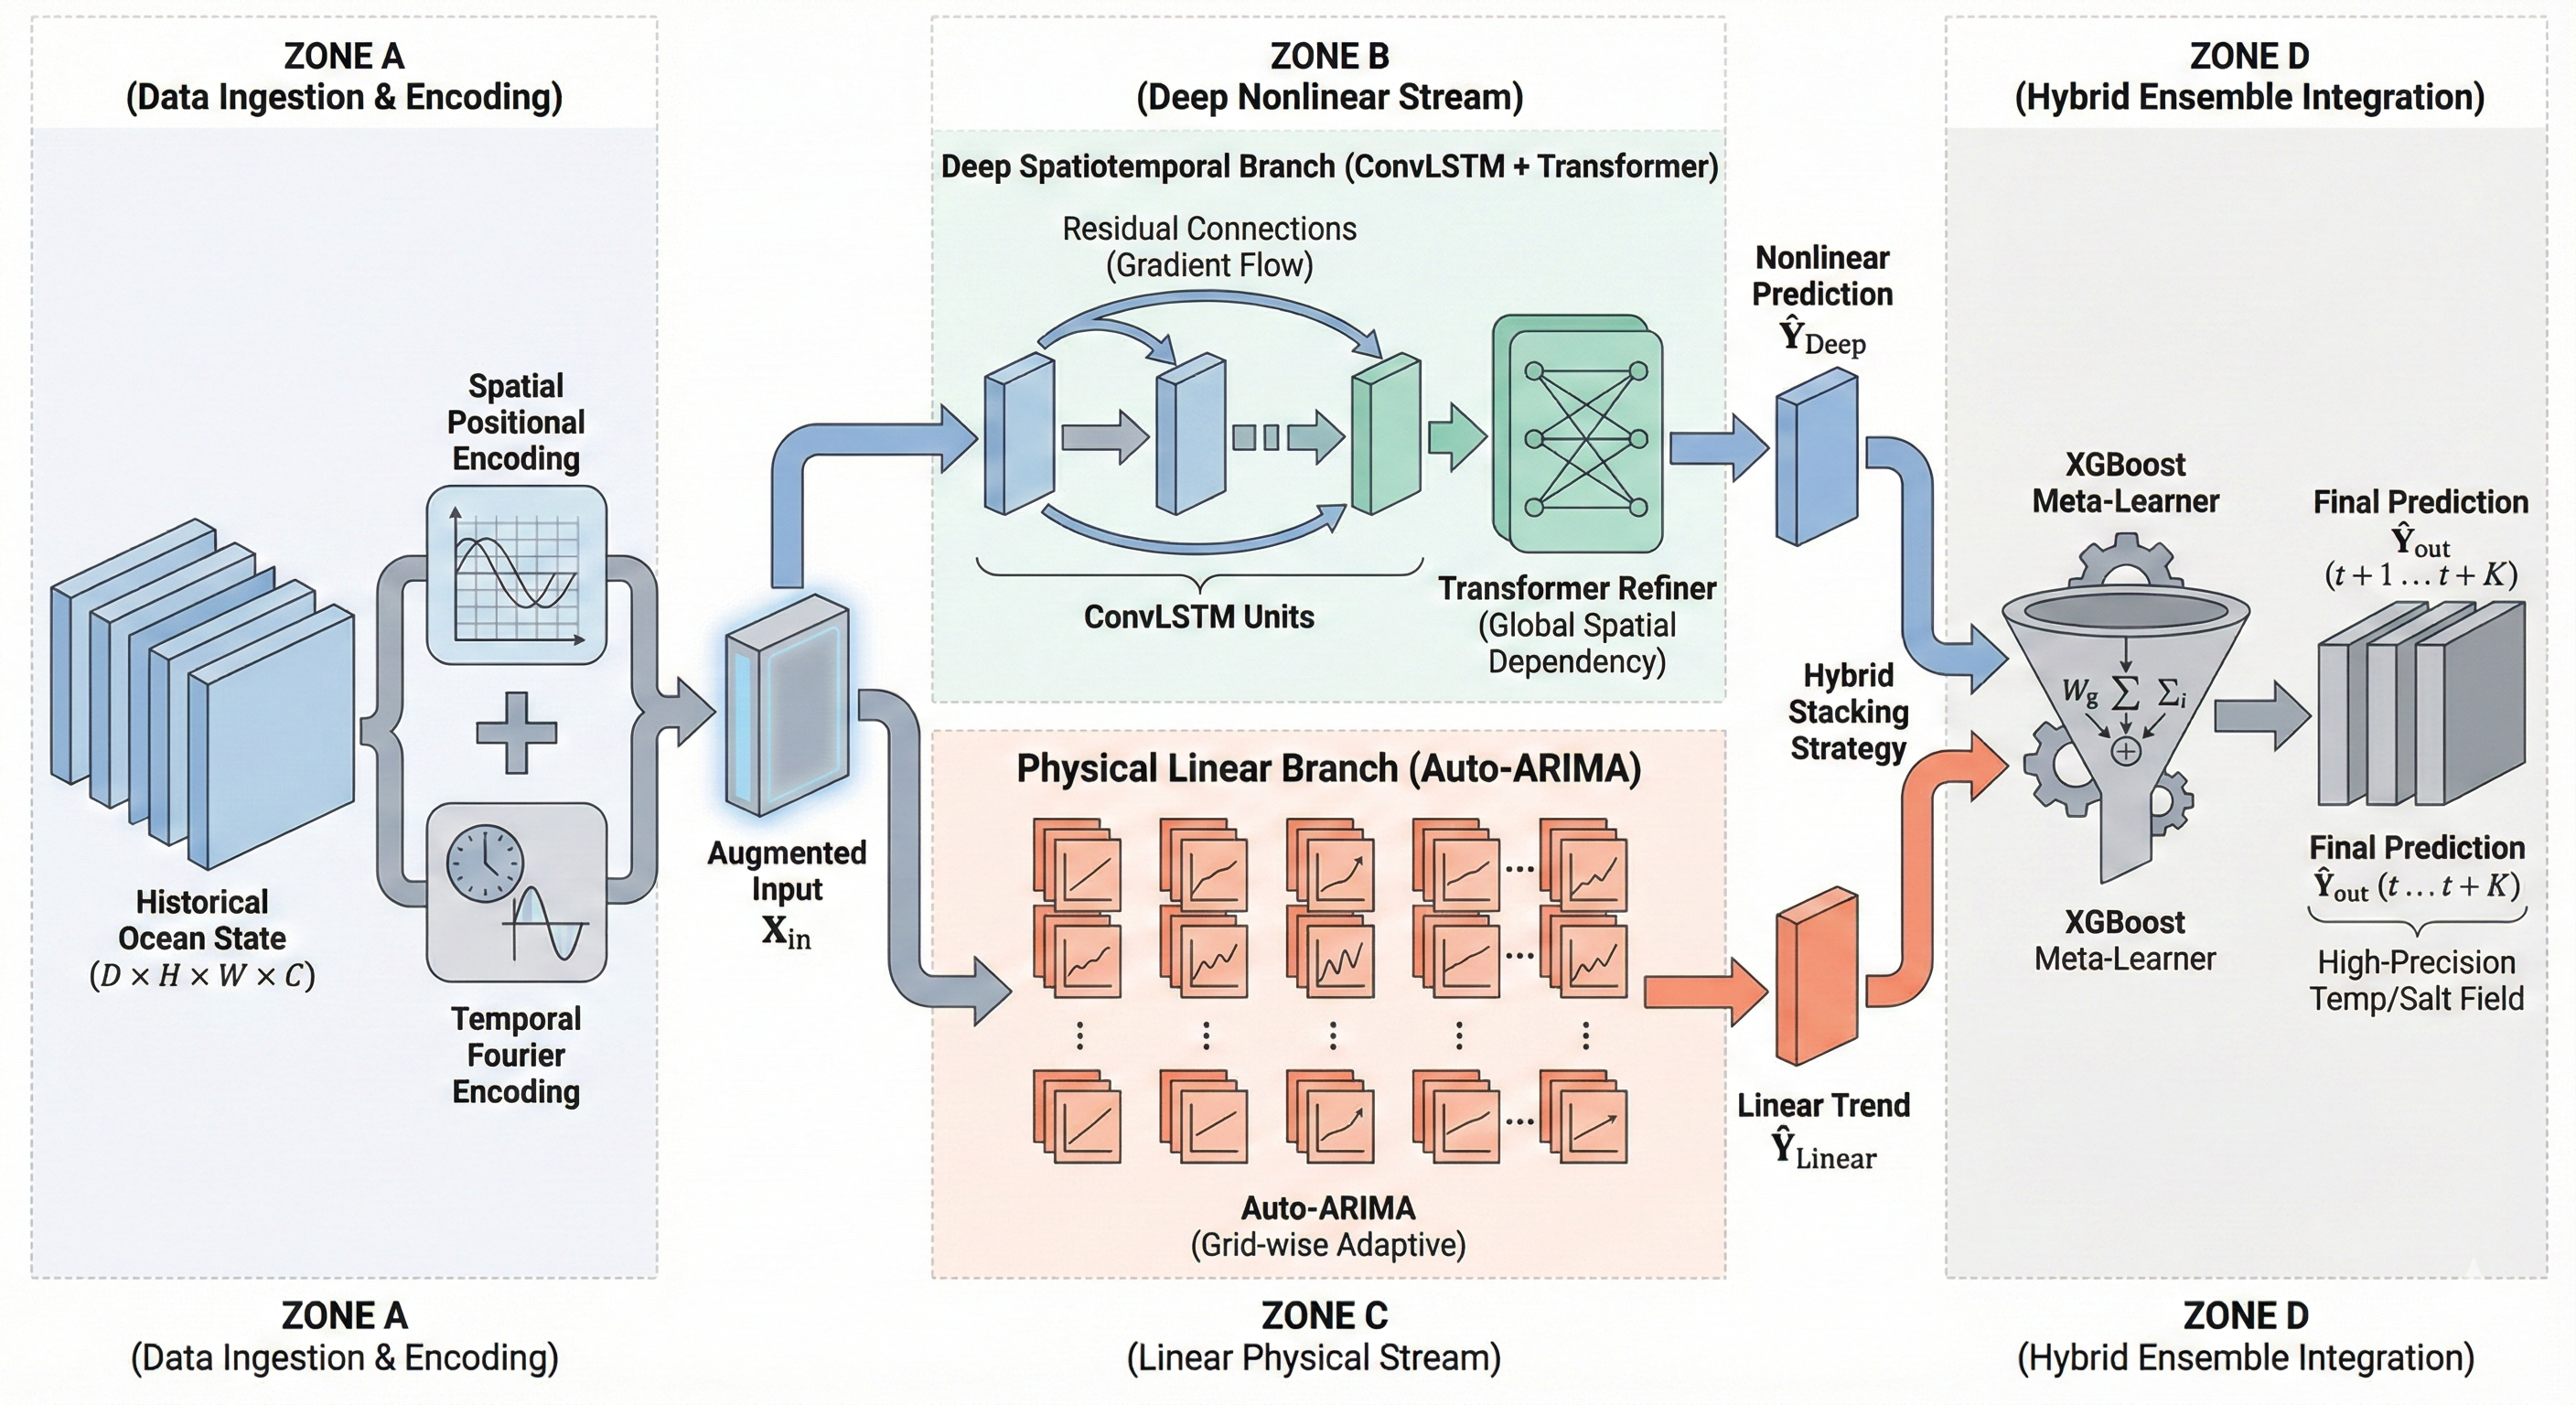
\includegraphics[width=\linewidth]{Gemini_Generated_Image_rlvclurlvclurlvc.png}
\caption{Model Architecture Diagram}
\label{fig:model_arch}
\end{figure*}

\subsubsection{Spatiotemporal Feature Encoding}

This study designed and adopted a spatiotemporal encoding module which maps longitude, latitude, depth, and time into high-dimensional feature vectors, and cascades them with other physical state variables as channels to serve as the enhanced input of the model $X_{in} \in \mathbb{R}^{T \times (C_{phy} + C_{enc}) \times H \times W}$.

\paragraph{Spatial Positional Encoding}

Traditional Convolutional Neural Networks (CNNs) have the characteristic of translation invariance. However, since the physical laws of the ocean have geographical dependencies, this causes CNNs to exhibit the defect of being unable to perceive absolute ocean positions in ocean temperature and salinity prediction. To solve this defect, this study introduces a spatial positional encoding scheme based on sine and cosine functions, and through the design of multi-frequency components, enables the model to capture multi-scale spatial dependencies. The specific steps are as follows:

Represent the spatial grid points in radians as $(lon, lat)$. Then, construct an encoding vector containing $N_s$ frequency components:

For position $p \in \{lon,lat\}$, the encoding formula for the $k$-th frequency component ($k=0, \dots, N_s-1$) is defined as:

\begin{equation}
\begin{aligned}
PE_{(p, 2k)} &= \sin\left(\frac{p}{10000^{k/N_s}}\right) \\
PE_{(p, 2k+1)} &= \cos\left(\frac{p}{10000^{k/N_s}}\right)
\end{aligned}
\end{equation}

The encoding vectors for longitude and latitude are concatenated in the feature dimension to form a spatial feature map with a total dimension of $4N_s$.

\paragraph{Temporal Fourier Encoding}

Since 2D ConvLSTM usually simply concatenates the time variable as a channel variable, it lacks intrinsic perception of "time" as a physical coordinate. However, the ocean temperature and salinity fields have obvious seasonal time periodicity, and a monotonically increasing time variable is obviously unfavorable for the model to capture periodic information. To explicitly model this periodicity, the encoding scheme adopts a temporal encoding technique based on Fourier series, intended to capture the high-frequency cycle of ocean interannual seasonal fluctuations through Fourier series, while combining normalized year term information to characterize the low-frequency linear long-term climate change trend. The specific steps are as follows:

For the month $m_t \in [0, 11]$ corresponding to time step $t$, taking $T_{period}=12$ as the reference period, calculate the $N_t$-order harmonic components:

\begin{equation}
\begin{aligned}
TE_{(t, 2k)} &= \sin\left(\frac{2\pi \cdot m_t \cdot (k+1)}{T_{period}}\right) \\
TE_{(t, 2k+1)} &= \cos\left(\frac{2\pi \cdot m_t \cdot (k+1)}{T_{period}}\right)
\end{aligned}
\end{equation}

In addition, to capture the non-stationary long-term climate change trend, we introduced a normalized year trend term:

\begin{equation}
Y_{norm} = (year_t - year_{min}) / (year_{max} - year_{min})
\end{equation}

The final temporal encoding fuses periodic features and linear trend features, allowing the model to capture both seasonal fluctuations and adapt to interannual changes.

\subsubsection{ConvLSTM Unit}

To effectively achieve spatiotemporal modeling of ocean temperature and salinity fields, inspired by the pioneering work of Shi et al. \cite{shiConvolutionalLSTMNetwork2015} introducing convolutional structures into recurrent neural networks, and the application of deep spatiotemporal models in the field of ocean element prediction by scholars such as Xiao \cite{xiaoSpatiotemporalDeepLearning2019}, this study selects the Convolutional LSTM network (ConvLSTM) as the backbone network for spatiotemporal feature extraction. Relevant studies, such as the application of CNN for multi-year ENSO forecasts \cite{hamDeepLearningMultiyear2019} and the use of spatiotemporal LSTMs for predictive learning \cite{wangPredRNNRecurrentNeural2017}, show that deep learning models can capture complex nonlinear features in the ocean dynamic environment through end-to-end learning. ConvLSTM replaces the fully connected layer of standard LSTM with convolution operations, avoiding the destruction of spatial neighborhood relationships of complex ocean temperature and salinity data by tensor flattening in fully connected operations. The convolution operation naturally preserves the spatial topological structure information of the input tensor through its local receptive field based on preserving input spatial topological structure information, thereby achieving effective spatiotemporal modeling.

The state update of the ConvLSTM unit at time step $t$ follows the following dynamic equations:

\begin{equation}
\begin{aligned} i_t &= \sigma(W_{xi} * \mathcal{X}_t + W_{hi} * \mathcal{H}_{t-1} + W_{ci} \circ \mathcal{C}_{t-1} + b_i) \\ f_t &= \sigma(W_{xf} * \mathcal{X}_t + W_{hf} * \mathcal{H}_{t-1} + W_{cf} \circ \mathcal{C}_{t-1} + b_f) \\ \mathcal{C}_t &= f_t \circ \mathcal{C}_{t-1} + i_t \circ \tanh(W_{xc} * \mathcal{X}_t + W_{hc} * \mathcal{H}_{t-1} + b_c) \\ o_t &= \sigma(W_{xo} * \mathcal{X}_t + W_{ho} * \mathcal{H}_{t-1} + W_{co} \circ \mathcal{C}_t + b_o) \\ \mathcal{H}_t &= o_t \circ \tanh(\mathcal{C}_t) \end{aligned}
\end{equation}

Where $\mathcal{X}_t$ is the temperature and salinity input field at the current moment, $\mathcal{H}_t$ is the hidden state, and $\mathcal{C}_t$ is the cell state. $*$ denotes convolution operation, and $\circ$ denotes Hadamard product.

In this structure, the forget gate ($f_t$) mainly regulates the retention degree of historical heat and salt memory ($\mathcal{C}_{t-1}$) to simulate the thermal inertia and persistence characteristics of the ocean physical system; the input gate ($i_t$) is responsible for controlling the inflow of information from the current moment observation data ($\mathcal{X}_t$) to the system state, reflecting the update and regulation effect of external forcing on the ocean environment state; the cell state ($\mathcal{C}_t$) acts as the core "memory flow" running through the time series, effectively maintaining the long-term dependence of spatiotemporal evolution of ocean temperature and salinity fields by accumulating and transmitting long-term evolution features.

Although ConvLSTM has excellent spatiotemporal modeling capabilities, it still faces problems such as gradient attenuation in deep networks and fixed convolution kernel weights in complex ocean temperature and salinity field modeling, leading to the model's inability to adaptively focus on learning extreme variation regions in the ocean environment. To overcome the above limitations, this paper further introduces improvement schemes of residual connections and multi-head attention mechanism based on standard ConvLSTM, and designs an ensemble strategy based on Stacking technology to construct a higher performance prediction architecture.

\subsubsection{Advanced Mechanisms \& Hybrid Strategy}

\paragraph{Residual Connections}

As the number of ConvLSTM network layers increases, gradient vanishing and exploding problems will significantly limit the training effect of the model, especially when processing long-sequence ocean spatiotemporal data, insufficient deep feature extraction will become a constraint for temperature and salinity field inversion. To alleviate this problem, this study introduced a residual connection mechanism between stacked ConvLSTM layers, allowing gradients to propagate directly from deep layers back to shallow layers, thereby ensuring stable training. Specifically, for the output $\mathcal{H}^l_t$ of the $l$-th layer, its calculation formula is:

\begin{equation}
\mathcal{H}^l_t = \mathcal{H}^{l-1}_t + f_l \bigl( \mathcal{H}^{l-1}_t,\; \mathcal{H}^l_{t-1},\; \mathcal{C}^l_{t-1} \bigr)
\end{equation}

Where $f_l(\cdot)$ represents the $l$-th layer ConvLSTM unit. This design preserves the low-order features of the original input while allowing the network to learn high-order residual mappings, avoiding information loss. 

\paragraph{Transformer Refiner}

To ensure computational efficiency, this study did not directly embed the attention mechanism inside the ConvLSTM unit, but designed the attention mechanism as a key refinement module. Through a two-stage strategy of extracting local spatiotemporal features + Transformer correcting global spatial dependencies, it effectively improved the model's ability to predict large-scale complex ocean phenomena while ensuring computational efficiency. Its core mechanism is to enhance the spatiotemporal consistency of the model output through a dedicated Transformer Refiner module after the ConvLSTM backbone network completes spatiotemporal feature extraction and decoding.

This module utilizes the powerful global modeling capability of Transformer to convert the two-dimensional ocean spatial field into a sequence signal for processing through three key steps: firstly, feature serialization, flattening the four-dimensional feature map $(B,C,H,W)$ output by ConvLSTM decoding in the spatial dimension into a sequence form of $(B, H \times W, C)$, where each pixel point $(H \times W)$ is regarded as an independent Token; secondly, performing global correlation calculation, using the self-attention mechanism to calculate the weight distribution between all pixel points pairwise, meaning the model will calculate the correlation between any point in the current sea area and all other points in the entire sea area; finally, the spatial reconstruction link, restoring the processed sequence features to the spatial feature map structure of $(B,C,H,W)$.

After introducing spatial self-attention, the model can "see" the whole picture, enabling the prediction of a certain place to rely not only on its neighborhood but also refer to distant ocean states, making the predicted temperature/salinity field smoother in spatial distribution and consistent with physical laws. 

\paragraph{Ensemble Strategy}

Ocean temperature and salinity field data often contain both significant linear trends (such as seasonal cycles, long-term warming trends, and tidal driving) and complex nonlinear dynamic processes. It is difficult for a single model to capture these two types of features efficiently at the same time. Therefore, this paper designs a linear and nonlinear hybrid ensemble strategy based on Stacking technology, fully mining the complementary advantages of different models through multi-level fusion.

This strategy specifically includes the following three core parts working in synergy:

First is the Linear Component. Aiming at the problem that a single fixed model order is difficult to adapt to the dynamic characteristics of all grid points, this paper abandons the traditional fixed parameter strategy and introduces the Auto-ARIMA automatic order determination mechanism to independently model the time series of each spatial grid point. This mechanism uses Grid Search to adaptively determine the optimal non-seasonal parameters $(p,d,q)$ and seasonal parameters $(P,D,Q)_s$ for each grid. The model selection process is based on the Akaike Information Criterion (AIC) minimization principle:

\begin{equation}
\text{Minimize } \text{AIC} = 2k - 2\ln(\hat{L})
\end{equation}

Where $k$ is the number of model parameters, and $\hat{L}$ is the maximum value of the likelihood function. By introducing seasonal differencing and adaptive parameter optimization, this module can accurately capture the linear trends, non-stationarity, and seasonal fluctuations specific to different sea areas, separating cleaner residual signals for subsequent nonlinear modeling.

Second is the Nonlinear Component, using the aforementioned enhanced ConvLSTM network (integrating residual connections and attention refinement module) as the backbone, responsible for modeling complex spatiotemporal nonlinear evolution processes, focusing on capturing high-frequency strong convection phenomena such as eddy migration, front movement, and rapid temperature changes induced by typhoons.

Finally, the Stacking Meta-learner, introducing XGBoost as a second-level meta-learner to achieve adaptive fusion of linear and nonlinear prediction values. Specifically, the prediction values of ConvLSTM and Auto-ARIMA at the same time and the same grid point are constructed as feature vectors $\mathbf{X}_{\text{meta}}$:

\begin{equation}
\mathbf{X}_{\text{meta}} = \left[ \hat{Y}_{\text{ConvLSTM}}, \hat{Y}_{\text{Auto-ARIMA}} \right]
\end{equation}

XGBoost uses the true observation value $Y_{true}$ as the supervision target to learn the optimal combination mapping $f_{\text{XGBoost}}$ of the two. Benefiting from Auto-ARIMA's fine extraction of local linear features, the Stacking module can focus more on correcting nonlinear errors.

After introducing this module, in the temperature and salinity field prediction of this project, compared with the basic ConvLSTM model, the RMSE of \textbf{Temperature (TEMP)} is reduced by \textbf{16.5\%}, and the RMSE of \textbf{Salinity (SALT)} is reduced by \textbf{64.7\%}; compared with the traditional CNN benchmark model, the RMSE of \textbf{Temperature} is reduced by \textbf{42.4\%}, and the RMSE of \textbf{Salinity} is reduced by \textbf{71.9\%}.

\section{Experimental Setup}

\subsection{Experimental Environment and Model Training Configuration}

The model training and validation in this study were carried out on a high-performance computing platform. The hardware core adopts the \textbf{NVIDIA GeForce RTX 5090 GPU} with high-performance tensor computing capabilities, and the software environment is built based on the \textbf{PyTorch 2.8.0} framework, combined with \textbf{CUDA 12.8} to achieve underlying parallel acceleration. In the data processing flow, in addition to using NumPy and Xarray for conventional tensor operations, the oceanographic standard library \textbf{gsw (Gibbs SeaWater)} was introduced to ensure the rigor of temperature and salinity physical quantity conversion.

In terms of training strategy, this study set the initial learning rate to $1.57 \times 10^{-4}$ through Grid Search, and adopted a Batch Size of 8 to balance memory load and gradient estimation stability. Currently, the \textbf{Adam optimizer} is used for parameter optimization, supplemented by weight decay with a coefficient of $1\times 10^{-4}$ to suppress overfitting risk. To improve the model's ability to approach the global optimal solution in the later stage of training, a \textbf{ReduceLROnPlateau} dynamic scheduling strategy was introduced: by monitoring the validation set loss in real-time, when it does not decrease significantly within 10 consecutive Epochs, the learning rate is automatically decayed to 0.5 times the original. The overall training process was executed for 20 Epochs, ensuring that the model maintains good generalization performance while fully converging.

\subsection{Comprehensive Evaluation Metrics System}

To uniformly quantify the model's ability to restore the complex dynamics of ocean temperature and salinity fields, this paper constructs a comprehensive evaluation system combining \textbf{basic statistical metrics} and \textbf{physical derived consistency metrics}. At the basic statistical level, Root Mean Square Error (RMSE), Mean Absolute Error (MAE), and Coefficient of Determination ($R^2$) are used to evaluate the accuracy of the model in temperature and salinity scalar prediction.

Considering the constraints of ocean physical processes, this study further introduced physical derived variable evaluation based on the \textbf{TEOS-10} standard. Using the predicted temperature and salinity fields, calculated \textbf{Potential Density and Spiciness}, and compared them with the physical fields derived based on observed truth values. Among them, the accuracy of potential density directly reflects the model's reconstruction level of seawater vertical stratification structure and static stability (avoiding density inversion); spiciness serves as a state variable on isopycnal surfaces, used to measure the model's ability to maintain T-S relations and water mass characteristics. By calculating the error between the predicted derived field and the true derived field (such as $\text{RMSE}_{pden}$), this paper aims to reveal whether the model follows intrinsic thermodynamic constraints on the basis of numerical fitting, thereby ensuring that the prediction results have oceanographic rationality.

\section{Results and Analysis}

\subsection{Prediction Accuracy Analysis of Temperature and Salinity Fields}

We evaluated the prediction accuracy of the proposed model in terms of sea surface temperature (TEMP) and salinity (SALT). Through quantitative metrics such as Root Mean Square Error (RMSE) and Mean Absolute Error (MAE), the model's ability to effectively capture spatiotemporal dynamics was demonstrated.

During testing, the sliding window data augmentation strategy of this paper was turned off, and the test set samples were all selected from the raw data within the range of longitude 130.5°E–162.5°E, latitude 6.5°N–27.5°N, and depth covering 0–1000 m in the dataset constructed in this paper. The test set only includes the last 20\% time period, ensuring no intersection with the training set, preventing data leakage.

\subsubsection{Quantitative Performance Evaluation}

This section uses the trained Benchmark CNN, Basic ConvLSTM, and our final model to predict the test set data respectively. This work is based on standardized data. After converting the prediction results output by the model and the true values provided by the data loader to float64 precision, the prediction RMSE, MAE, and R² results for the 24 months included in the test set were directly calculated for the three models. The specific results are shown in the table below.

\begin{table}[H]
\caption{Comparison of Prediction Results of Different Models}
\centering
\resizebox{\linewidth}{!}{
\begin{tabular}{lllll}
\toprule
\textbf{Variable} & \textbf{Model Config} & \textbf{RMSE} & \textbf{MAE} & \textbf{R²} \\
\midrule
\textbf{TEMP} & Baseline CNN & 0.1513 & 0.1162 & 0.9773 \\
~ & Basic ConvLSTM & 0.1043 & 0.0833 & 0.9892 \\
~ & \textbf{Our Model (Stacking)} & \textbf{0.0871} & \textbf{0.0705} & \textbf{0.9925} \\
\textbf{SALT} & Baseline CNN & 0.4726 & 0.3533 & 0.7918 \\
~ & Basic ConvLSTM & 0.3763 & 0.2695 & 0.8680 \\
~ & \textbf{Our Model (Stacking)} & \textbf{0.1327} & \textbf{0.1041} & \textbf{0.9105} \\
\bottomrule
\end{tabular}
}
\end{table}

The results show that although the benchmark model has achieved an excellent score of $R^2$ > 0.97 in temperature, the temperature prediction effect of the Stacking model in this paper is still further improved. In terms of prediction accuracy, its RMSE reached 0.0871, which is reduced by 42.4\% compared to the Baseline CNN model (0.1513) and reduced by 16.5\% compared to the Basic ConvLSTM model (0.1043); in terms of fitting degree, $R^2$ is further improved to 0.9925, achieving the best fitting performance. In salinity prediction, the Stacking model in this paper still achieved excellent improvement effects: RMSE is 0.1327, reduced by about 71.9\% compared to Baseline CNN (0.4726); reduced by about 64.7\% compared to Basic ConvLSTM (0.3763), and $R^2$ is also significantly improved to 0.9105, making the salinity prediction fitting reach a highly accurate level.

\subsubsection{Visualization and In-Depth Analysis of Prediction Fields}

To comprehensively evaluate the model's prediction performance, we performed detailed visualization analysis from four dimensions: spatial distribution, vertical structure, statistical bias, and temporal phase.

\paragraph{6.1.2.1. Spatial Distribution and Error Analysis}

Considering the strong geographical heterogeneity of ocean temperature and salinity fields, analyzing the spatial distribution of model predictions can directly observe whether the model captures subtle fluctuations at the horizontal level, and observe the model's degree of restoration of spatial gradients and eddy structures of temperature and salinity fields. The figure below shows the predicted fields, true fields, and their error distributions for temperature and salinity on representative test samples. The visualization data in this section are obtained by compressing and averaging the depth dimension and restoring the real physical values through inverse standardization, representing the average distribution map of temperature and salinity in all depth layers at this time step. Thus, the spatial distribution and model prediction effect of the overall ocean temperature and salinity fields can be observed.

From Figure \ref{fig:temp_compare}, it can be observed that the model basically restores the physical trend of the real ocean temperature field on a larger scale. Our model accurately restores the macro-spatial pattern of temperature decreasing from low latitude to high latitude in the study area. The error distribution is shown in Figure \ref{fig:temp_error}. In most sea areas, the prediction error is at a very low level ($\pm 0.75^\circ$C), maintaining high consistency with the real field. The model achieves the best prediction effect in areas with higher temperatures (concentrated in the middle of the image), while the error increases in areas with sharp temperature gradients. It can be considered that the model exhibits an over-smoothing state at the temperature front, that is, the model prediction shows a certain bias towards the mean effect, which means that the model has a risk of feature disappearance in frontal areas with sharp temperature changes. Overall, the prediction error of the improved model in this paper has achieved good performance, but there are still certain limitations in specific areas.

The prediction of the salinity field (Figure \ref{fig:salt_compare}) also shows high consistency with the real field, and the error remains at a very low level overall. From the error distribution (Figure \ref{fig:salt_error}), it is observed that unlike the phenomenon of increased frontal error shown in temperature, the error distribution of salinity prediction is more stable, and the prediction accuracy of the model does not decrease significantly even in areas where salinity (PSU) changes drastically. The main limitation of the model's salinity prediction appears in the upper left corner of the figure, that is, the southwest corner of the selected area. This area has many islands, and the salinity variable itself is affected by precipitation, runoff, and local dynamic processes, and the signal is more fragmented. Compared with other open ocean areas, this area may introduce more disturbance factors causing slight distortion in model prediction, but the overall error remains at a relatively accurate and acceptable level.

\begin{figure}[H]
\centering
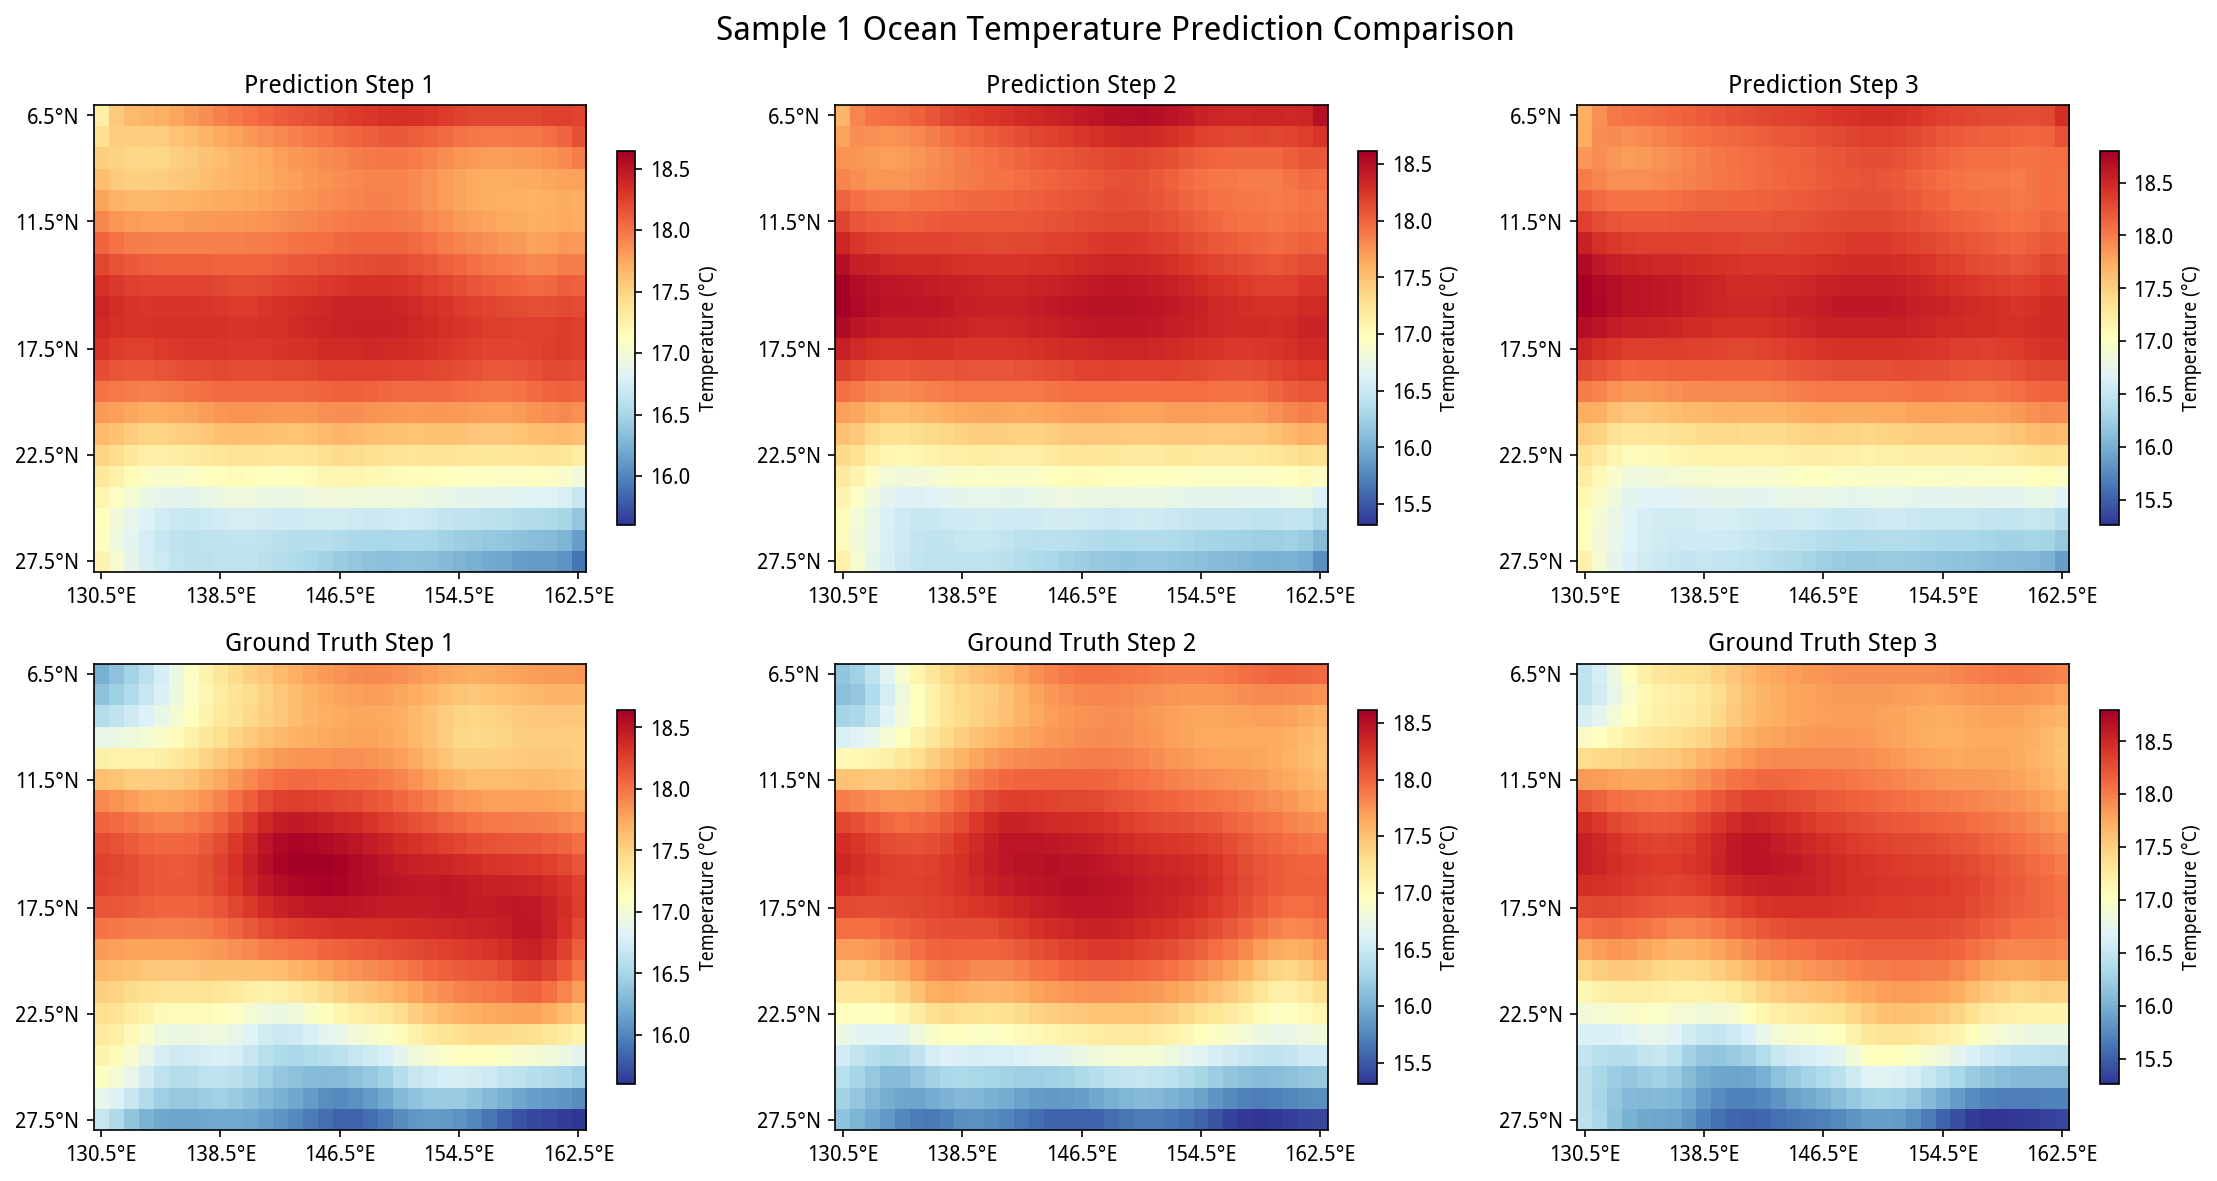
\includegraphics[width=\linewidth]{1765170625236-10.png}
\caption{Comparison of Predicted and True Temperature Fields}
\label{fig:temp_compare}
\end{figure}

\begin{figure}[H]
\centering
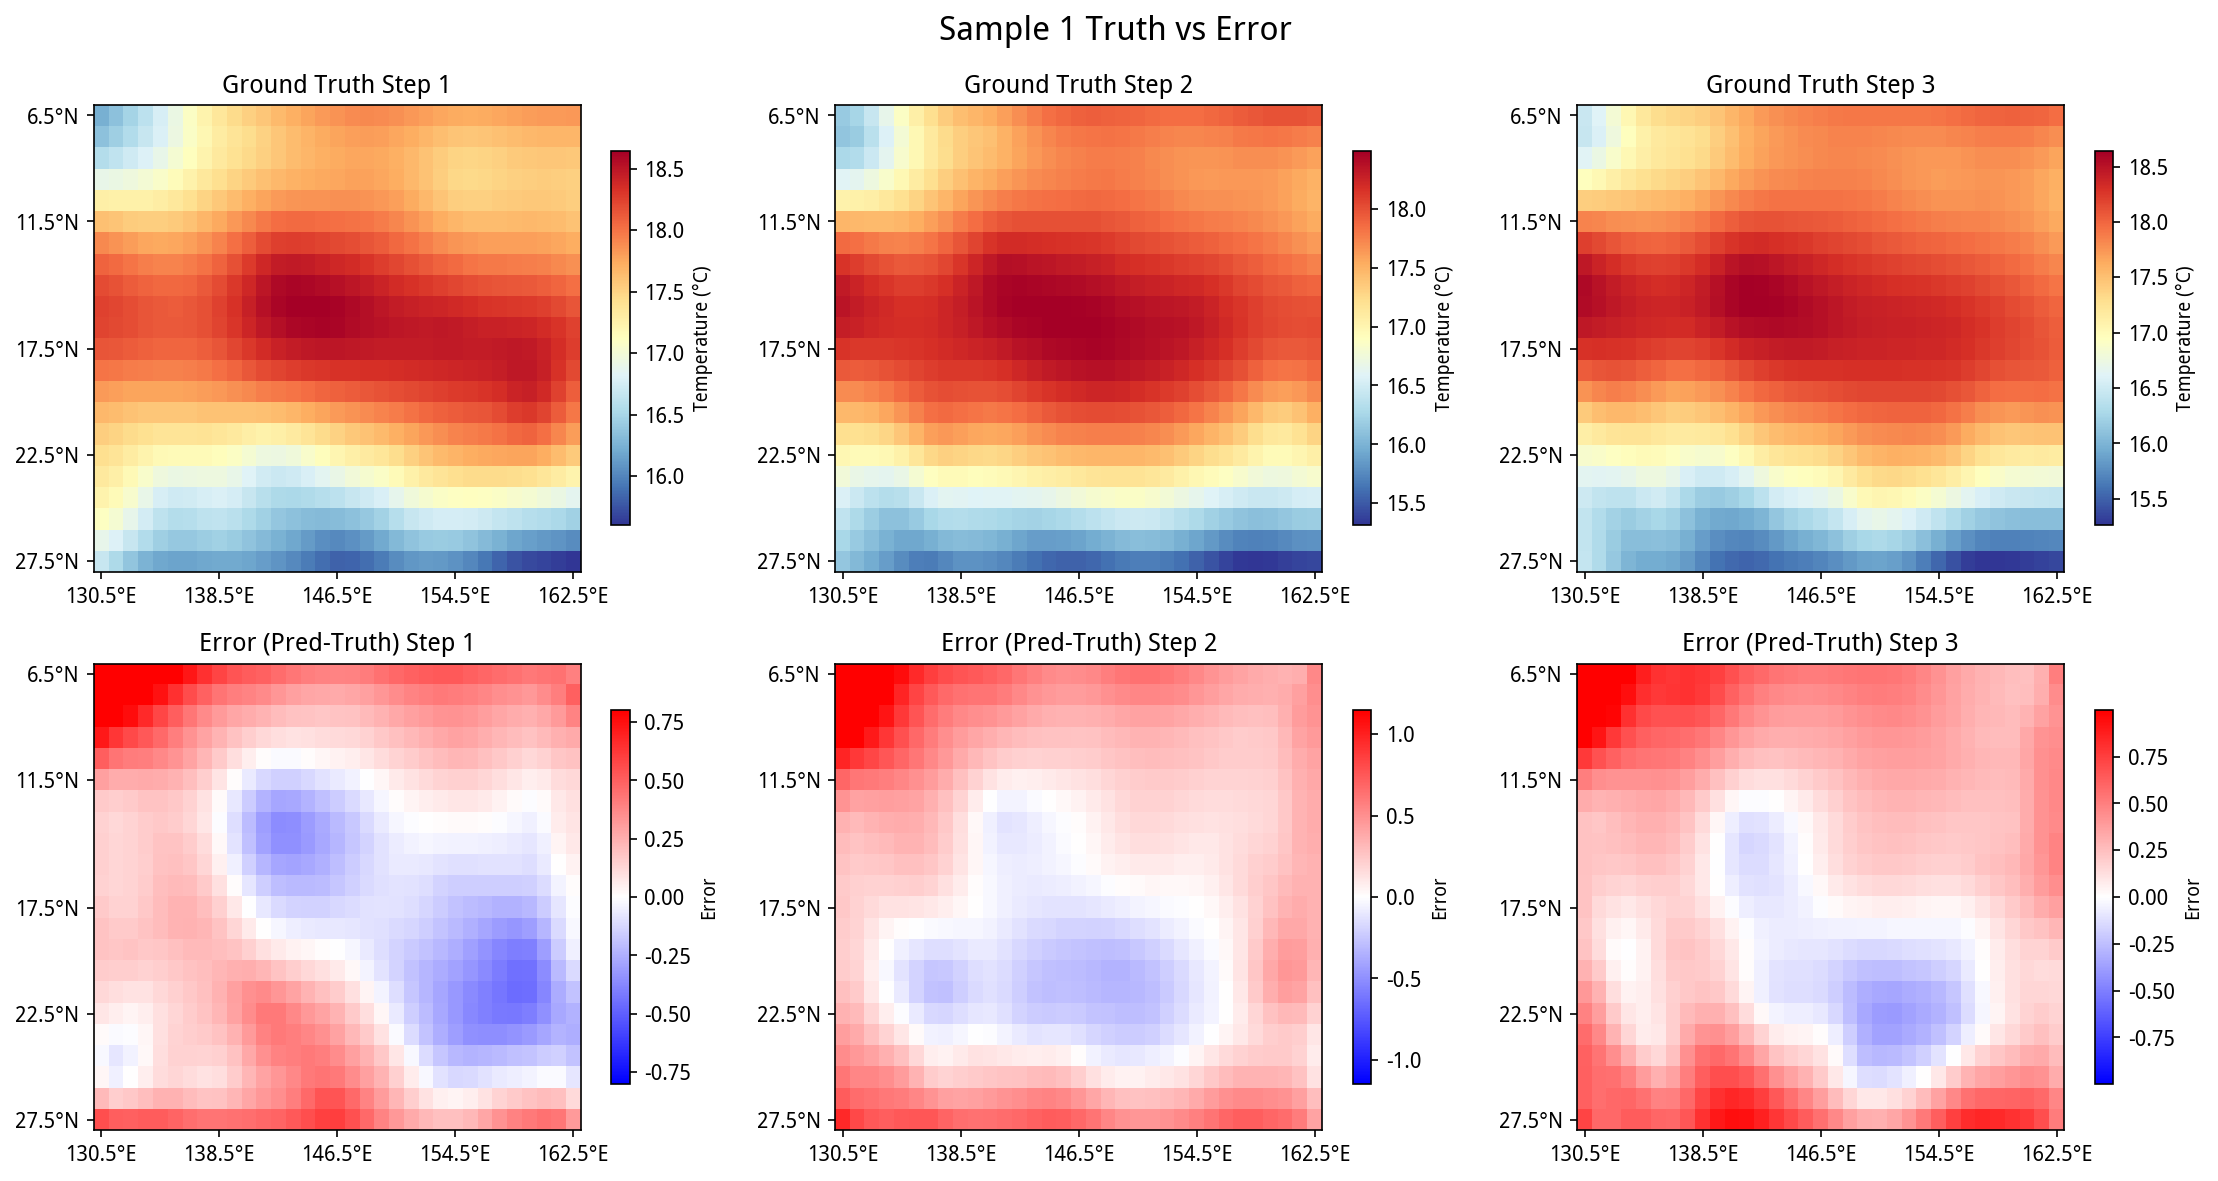
\includegraphics[width=\linewidth]{1765170627626-13.png}
\caption{Spatial Distribution of Temperature Prediction Errors}
\label{fig:temp_error}
\end{figure}

\begin{figure}[H]
\centering
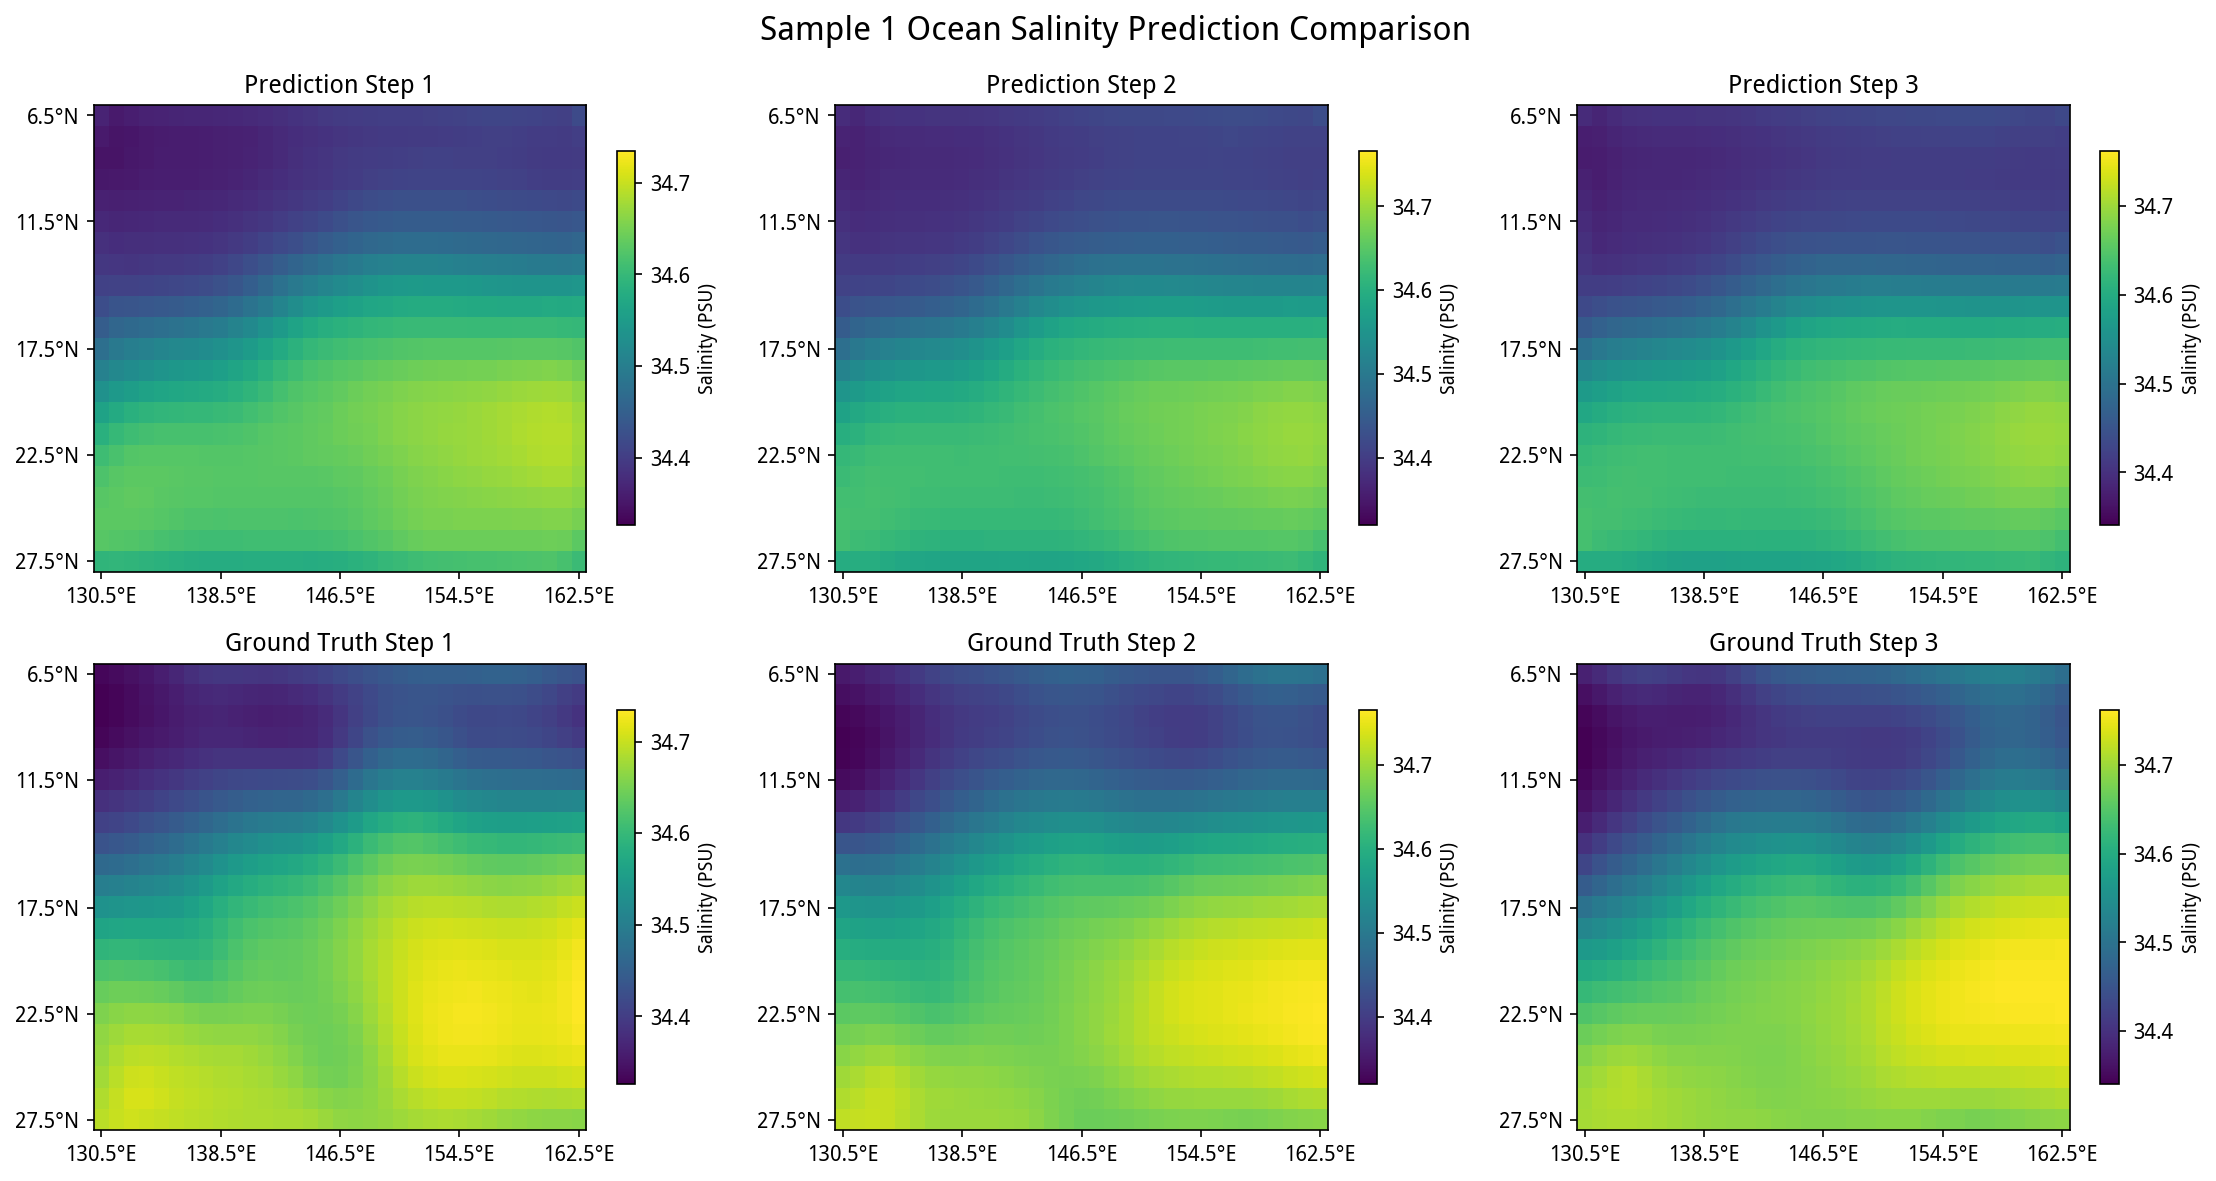
\includegraphics[width=\linewidth]{1765170631346-19.png}
\caption{Comparison of Predicted and True Salinity Fields}
\label{fig:salt_compare}
\end{figure}

\begin{figure}[H]
\centering
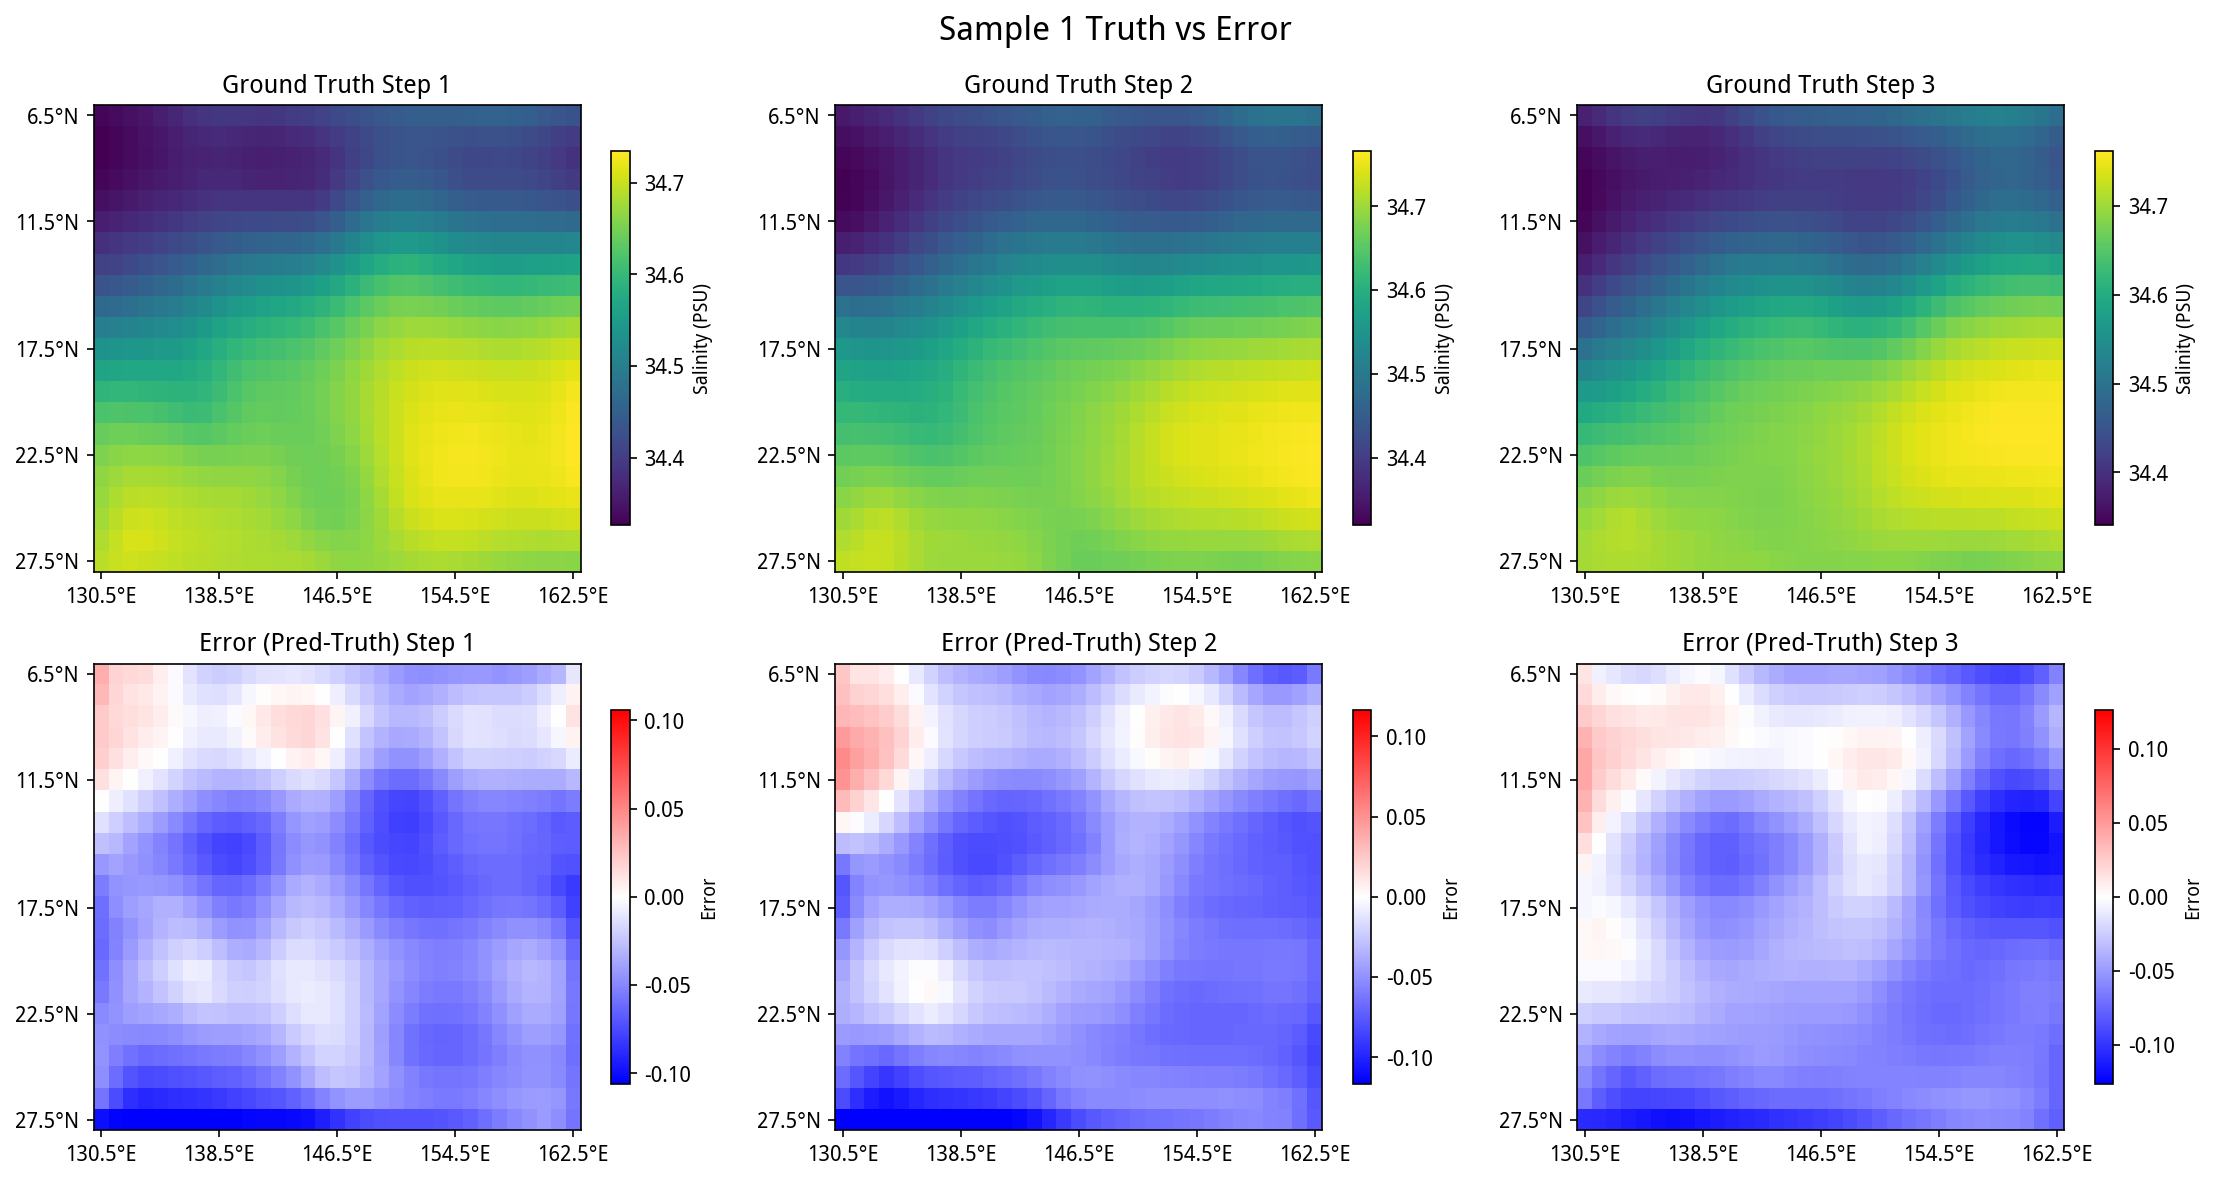
\includegraphics[width=\linewidth]{1765170629590-16.png}
\caption{Spatial Distribution of Salinity Prediction Errors}
\label{fig:salt_error}
\end{figure}

\paragraph{6.1.2.2. Depth Profile Analysis}

Accurately predicting the vertical structure is also an important link in ocean temperature and salinity field inversion. If the vertical structure prediction is distorted, it will lead to the "density inversion" phenomenon, violating physical laws. To verify the model's performance in the vertical direction, we plotted the depth profiles of predicted values and true values. The visualization data in this section comes directly from the model's inverse standardized prediction results and inverse standardized true values. By averaging each depth layer within the entire prediction area (latitude and longitude range), a depth profile map is generated to observe the model's vertical structure prediction effect, and the vertical structure prediction results under the model's prediction steps are displayed on the x-axis.

As shown in Figure \ref{fig:temp_profile} and Figure \ref{fig:salt_profile}, the model in this paper basically maintains the true vertical structure in the prediction of temperature and salinity. The predicted image and the real image maintain the true change trend, that is, temperature decreases with increasing depth, and salinity first increases and then decreases with increasing depth. From the perspective of error distribution, temperature prediction performs best in the first time step, and all depth layers show stable prediction effects. However, error accumulation appears in subsequent time steps, but the prediction from the subsurface to deeper layers (100.0m and below) still performs well. Salinity prediction does not show obvious error accumulation phenomenon with time steps. Its main error area is concentrated in the extreme value area of salinity (appearing near a depth of 150.0m), where the predicted value is lower than the true value, and the prediction in other areas maintains a stable and excellent prediction effect.

\begin{figure}[H]
\centering
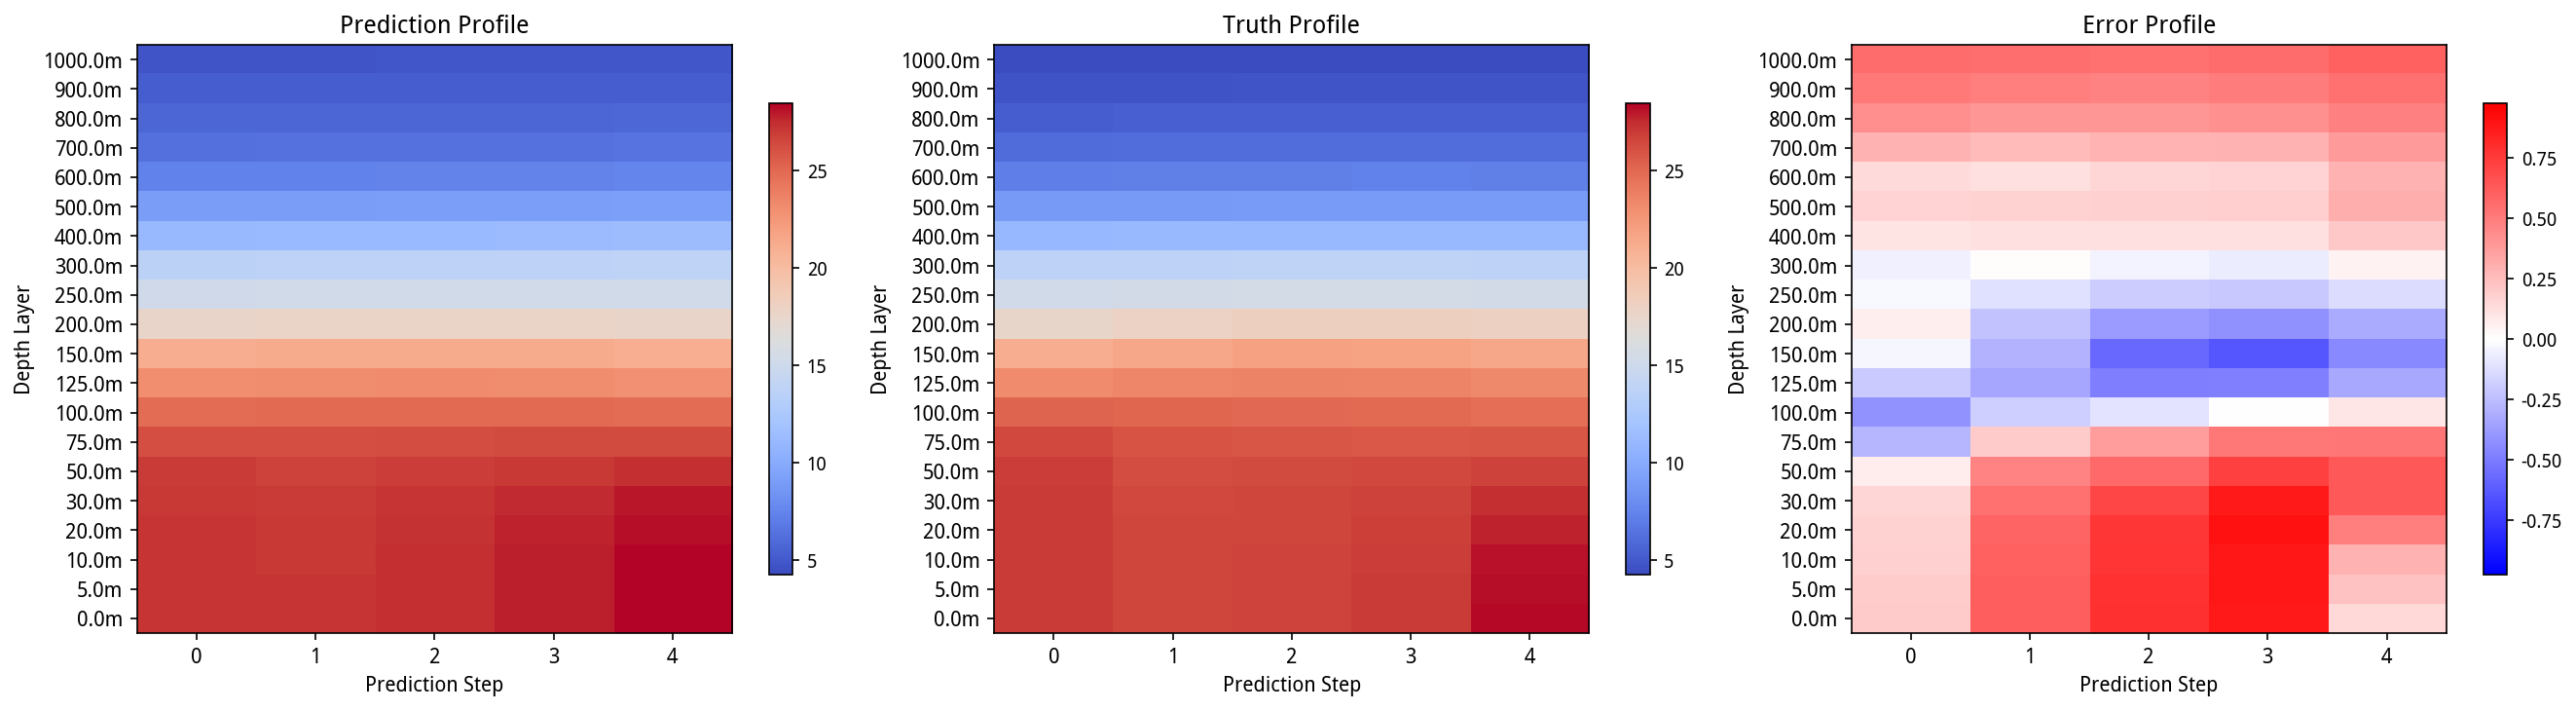
\includegraphics[width=\linewidth]{1765170641846-22.png}
\caption{Comparison of Temperature Depth Profile Predictions}
\label{fig:temp_profile}
\end{figure}

\begin{figure}[H]
\centering
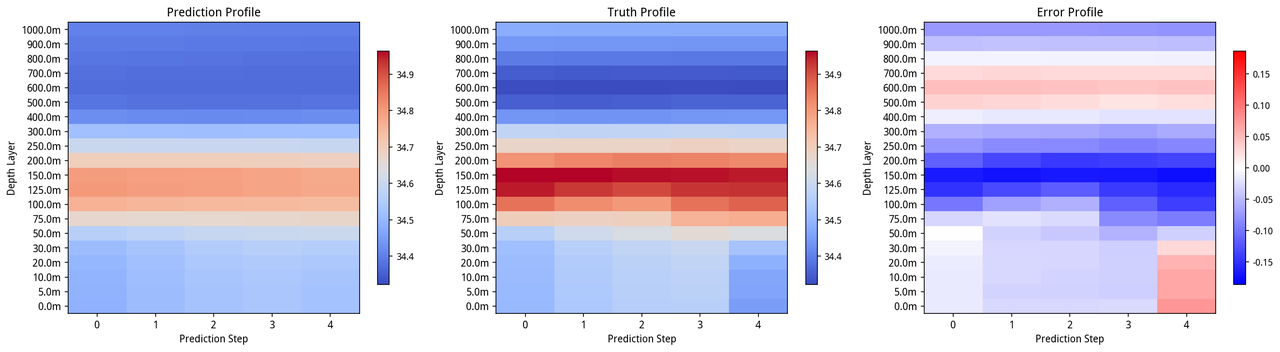
\includegraphics[width=\linewidth]{44ff20aa-c194-44f1-8800-3eaf2d3f7a5e.png}
\caption{Comparison of Salinity Depth Profile Predictions}
\label{fig:salt_profile}
\end{figure}

\paragraph{6.1.2.3. Statistical Bias Analysis}

To reflect the systematic error and dispersion of model prediction, we further analyzed the systematic bias of the model through scatter plots.

Scatter plots (Figure \ref{fig:scatter_plots}) show that the prediction points are closely distributed around the y=x diagonal, indicating that the model has no obvious systematic overestimation or underestimation. The fitting degree of temperature is extremely high (R² > 0.99), and although the dispersion of salinity is slightly larger, the overall trend is still accurate.

\begin{figure}[H]
\centering
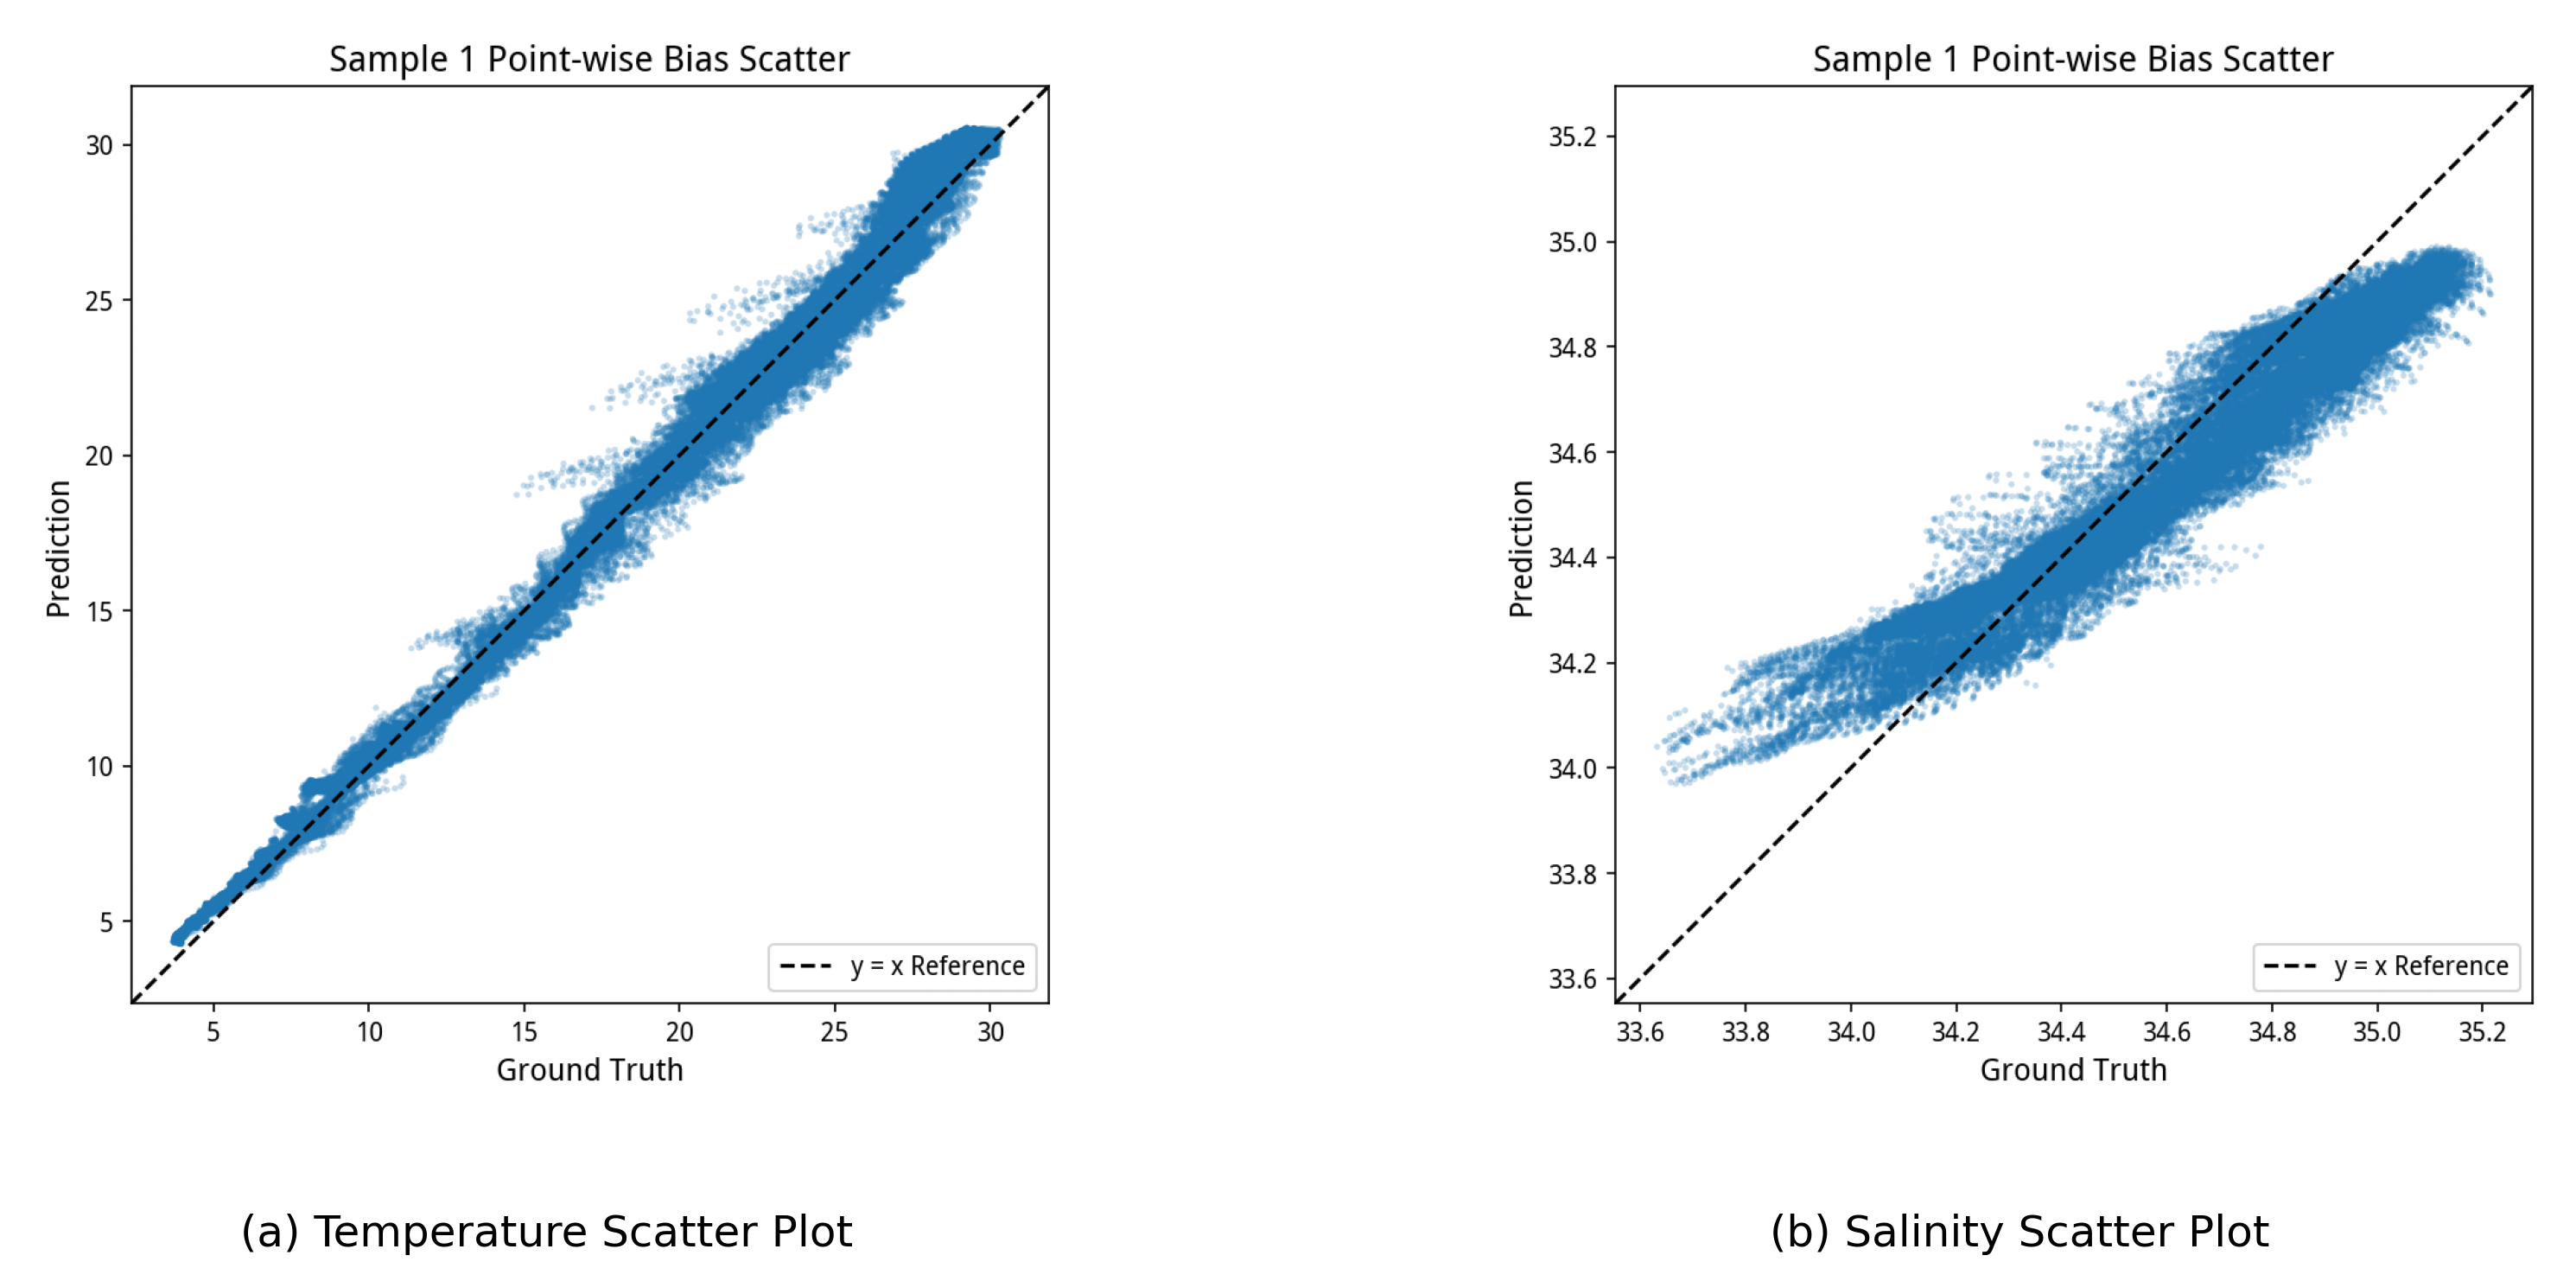
\includegraphics[width=\linewidth]{merged_scatter_plots.png}
\caption{Scatter Plots of Predicted vs True Values for Temperature (a) and Salinity (b)}
\label{fig:scatter_plots}
\end{figure}

\paragraph{6.1.2.4. Temporal Phase Error Analysis}

Finally, considering that ocean processes have significant periodicity (intraseasonal, seasonal, interannual) and lag effects, high prediction accuracy does not mean prediction success. If the warming/cooling trend predicted by the model lags on the time axis (i.e., phase error), the prediction result will lose value. Verifying phase consistency through Cross-correlation analysis ensures that the model has real-time response capability to changes in ocean temperature and salinity fields. First, calculate the spatial average values of temperature and salinity for the 3D temperature and salinity fields at each time step for the prediction results output by the model and the actual true values of the temperature and salinity fields in the dataset of this study, thereby generating two 1D time series based on the model prediction output, and performing standardization processing to preserve the trend information of the time series and strip off the influence of numerical absolute values. Then use the `np.correlate` function to calculate the correlation between the two sequences under different time lags.

Cross-correlation analysis (Figure \ref{fig:phase_error}) shows that the maximum correlation coefficient between the predicted sequence and the true sequence appears at a lag of 0 or 1, and the maximum correlation coefficients are all greater than 0.7. The coherence of temperature and salinity sequences decreases significantly with the increase of month delay, indicating that the model can well capture the change trends and fluctuation shapes of ocean temperature and salinity, without obvious lag phenomenon, showing excellent spatiotemporal consistency.

\begin{figure}[H]
\centering
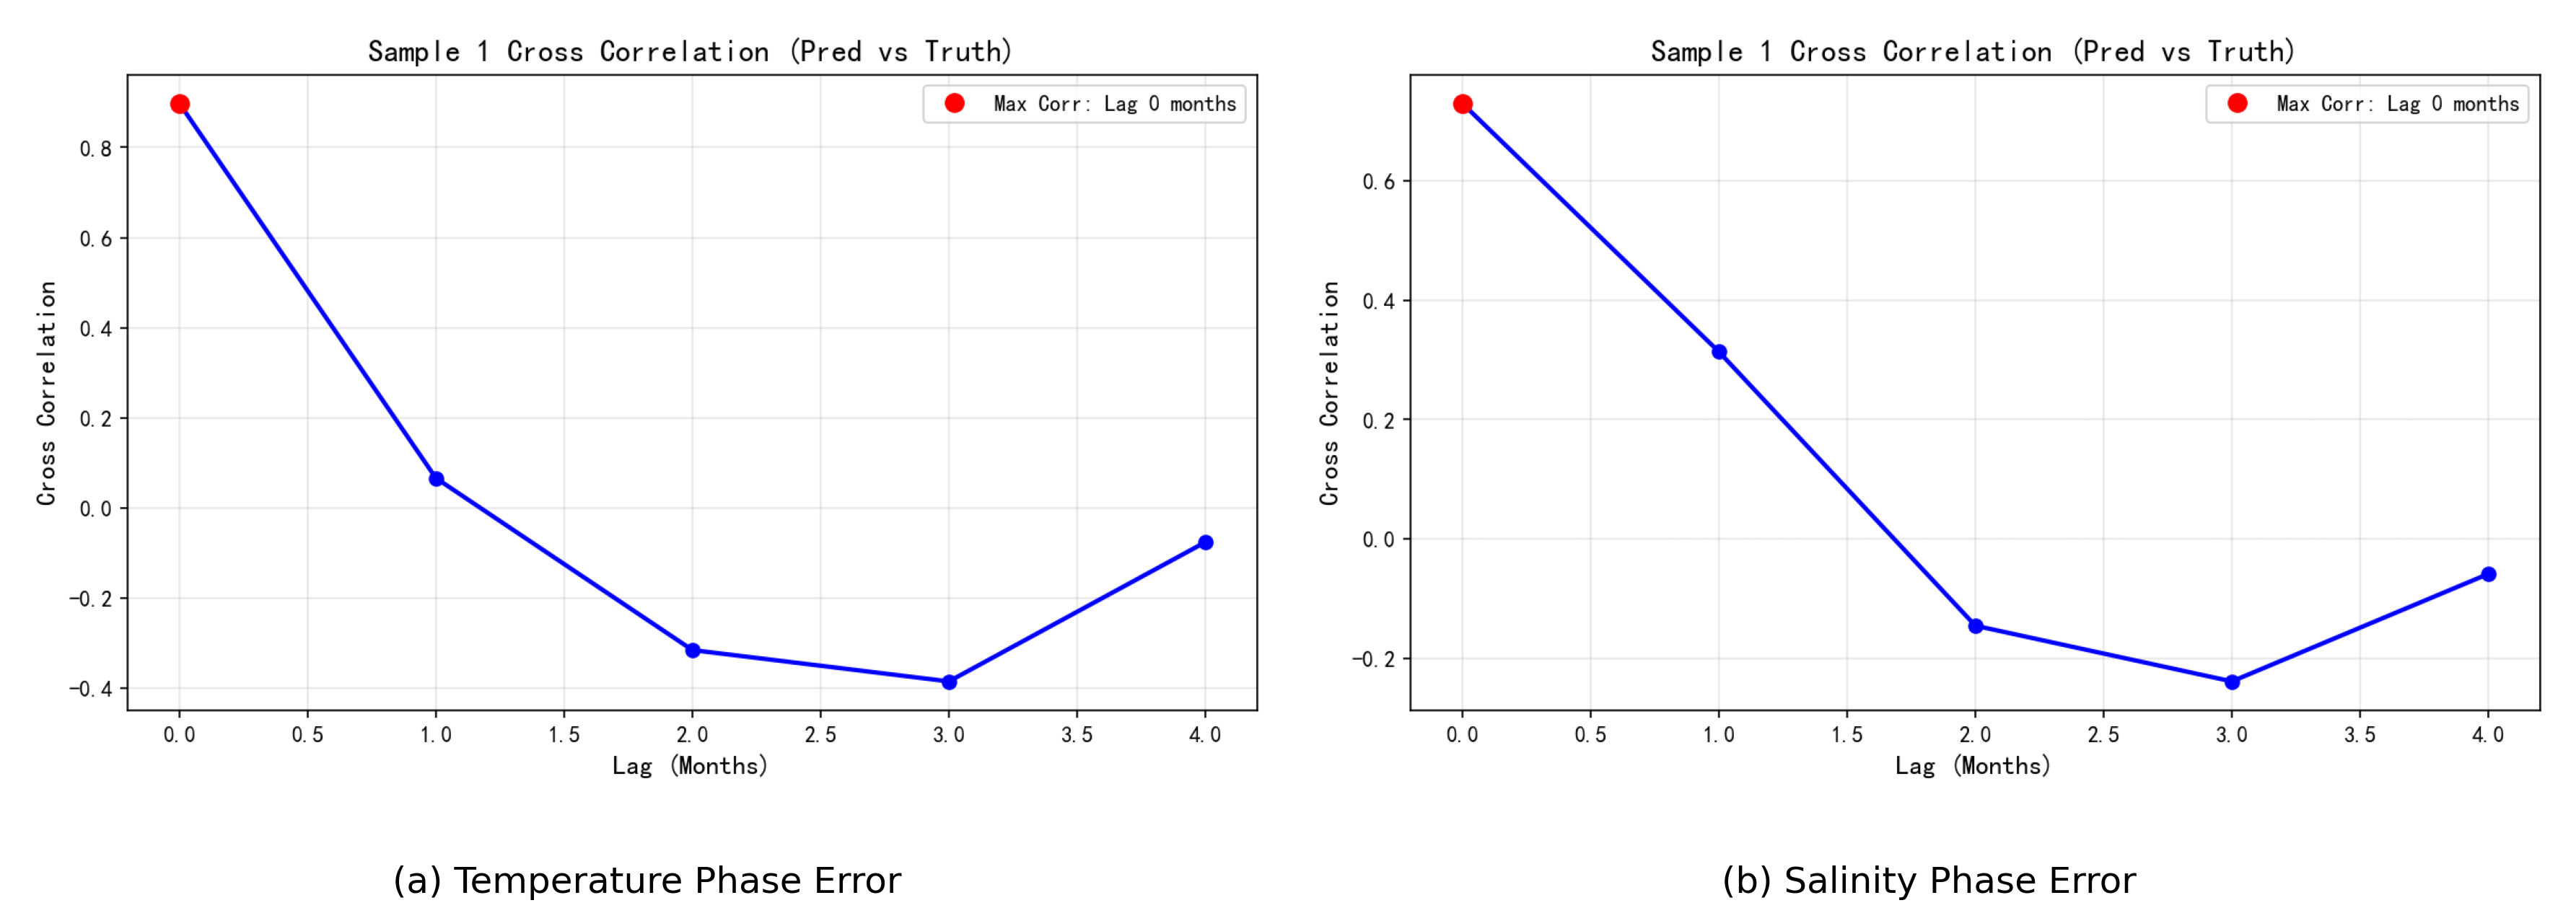
\includegraphics[width=\linewidth]{merged_phase_error_plots.png}
\caption{Cross-Correlation Analysis of Prediction Sequences for Temperature (a) and Salinity (b)}
\label{fig:phase_error}
\end{figure}

\subsection{Ablation Study}

We take the Standard CNN model and the Basic ConvLSTM model as two groups of benchmark models for reference, denoted as Model 1 and Model 2 respectively. Based on the Basic ConvLSTM model, Attention mechanism and Residual Connection are added respectively as Model 3 and Model 4; the model with only ARIMA-Stacking strategy added is denoted as Model 5; the ConvLSTM model with complete components (Attention + Residual) is denoted as Model 6 (Full); the model introducing ARIMA-Stacking ensemble strategy on the basis of Model 6 is denoted as Model 7 (Full + Stacking, the model finally selected in this paper). To validate specific modules, the model removing equatorial symmetry data augmentation on the basis of Model 7 is denoted as Model 8; the model removing sliding window data augmentation is denoted as Model 9; and the model removing spatiotemporal encoding is denoted as Model 10.

\subsubsection{Physical Consistency Assessment}

In addition to statistical accuracy, ensuring that the predicted fields maintain physical consistency is crucial. We evaluate this by deriving Potential Density (PDEN) and Spiciness (SPICE) from the predicted temperature and salinity fields using the TEOS-10 equation of state.

The table below shows the comparison of derived variable accuracy between the Stacking model (Model 7), the Benchmark model (Model 1), and the Basic ConvLSTM (Model 2).

\begin{table}[H]
\caption{Comparison of RMSE and MAE for Derived Physical Variables Under Different Model Configurations}
\centering
\resizebox{\linewidth}{!}{
\begin{tabular}{ccccc}
\toprule
\textbf{Metric} & \textbf{Variable} & \textbf{Baseline CNN} & \textbf{Basic ConvLSTM} & \textbf{Our Model} \\
\midrule
\textbf{RMSE} & PDEN & 0.4068 & 0.2668 & \textbf{0.2355} \\
~ & SPICE & 0.4968 & 0.3421 & \textbf{0.3227} \\
\textbf{MAE} & PDEN & 0.2871 & 0.1954 & \textbf{0.1766} \\
~ & SPICE & 0.3777 & 0.2779 & \textbf{0.2610} \\
\textbf{R²} & PDEN & 0.9654 & 0.9851 & \textbf{0.9884} \\
~ & SPICE & 0.9520 & 0.9772 & \textbf{0.9797} \\
\bottomrule
\end{tabular}
}
\end{table}

The RMSE of our model on PDEN and SPICE are \textbf{0.2355} and \textbf{0.3227} respectively, which are reduced by \textbf{42.1\%} and \textbf{35.0\%} respectively compared to Baseline CNN. In terms of MAE, PDEN and SPICE are reduced by \textbf{38.5\%} and \textbf{30.9\%} respectively. This indicates that the model can not only accurately predict single variables, but also well maintain the physical coupling relationship between variables. The $R^2$ values of the two derived variables both exceed \textbf{0.97} (PDEN reaches 0.9884), indicating that the predicted temperature and salinity fields can still highly restore the true distribution of physical properties after mapping through the nonlinear equation of state. The Stacking model (Model 7) consistently outperforms other configurations in terms of derived variables PDEN and SPICE, which indicates that the introduced ARIMA-Stacking error correction mechanism effectively optimizes the joint distribution of temperature and salinity properties. It not only demonstrates excellent performance in univariate prediction of temperature and salinity, but also maintains excellent comprehensive physical consistency.

\subsubsection{Quantitative Metric Analysis}

To understand the contribution of each component, this section analyzes the effects of the attention mechanism, residual connection mechanism, data augmentation, and positional encoding based on the metric information in Tables \ref{tab:ablation_r2}, \ref{tab:ablation_rmse}, and \ref{tab:ablation_mae}. Figure \ref{fig:ablation_radar} illustrates the performance of various improvement components on the three core metrics: R², RMSE, and MAE.

\begin{figure}[htbp]
\centering
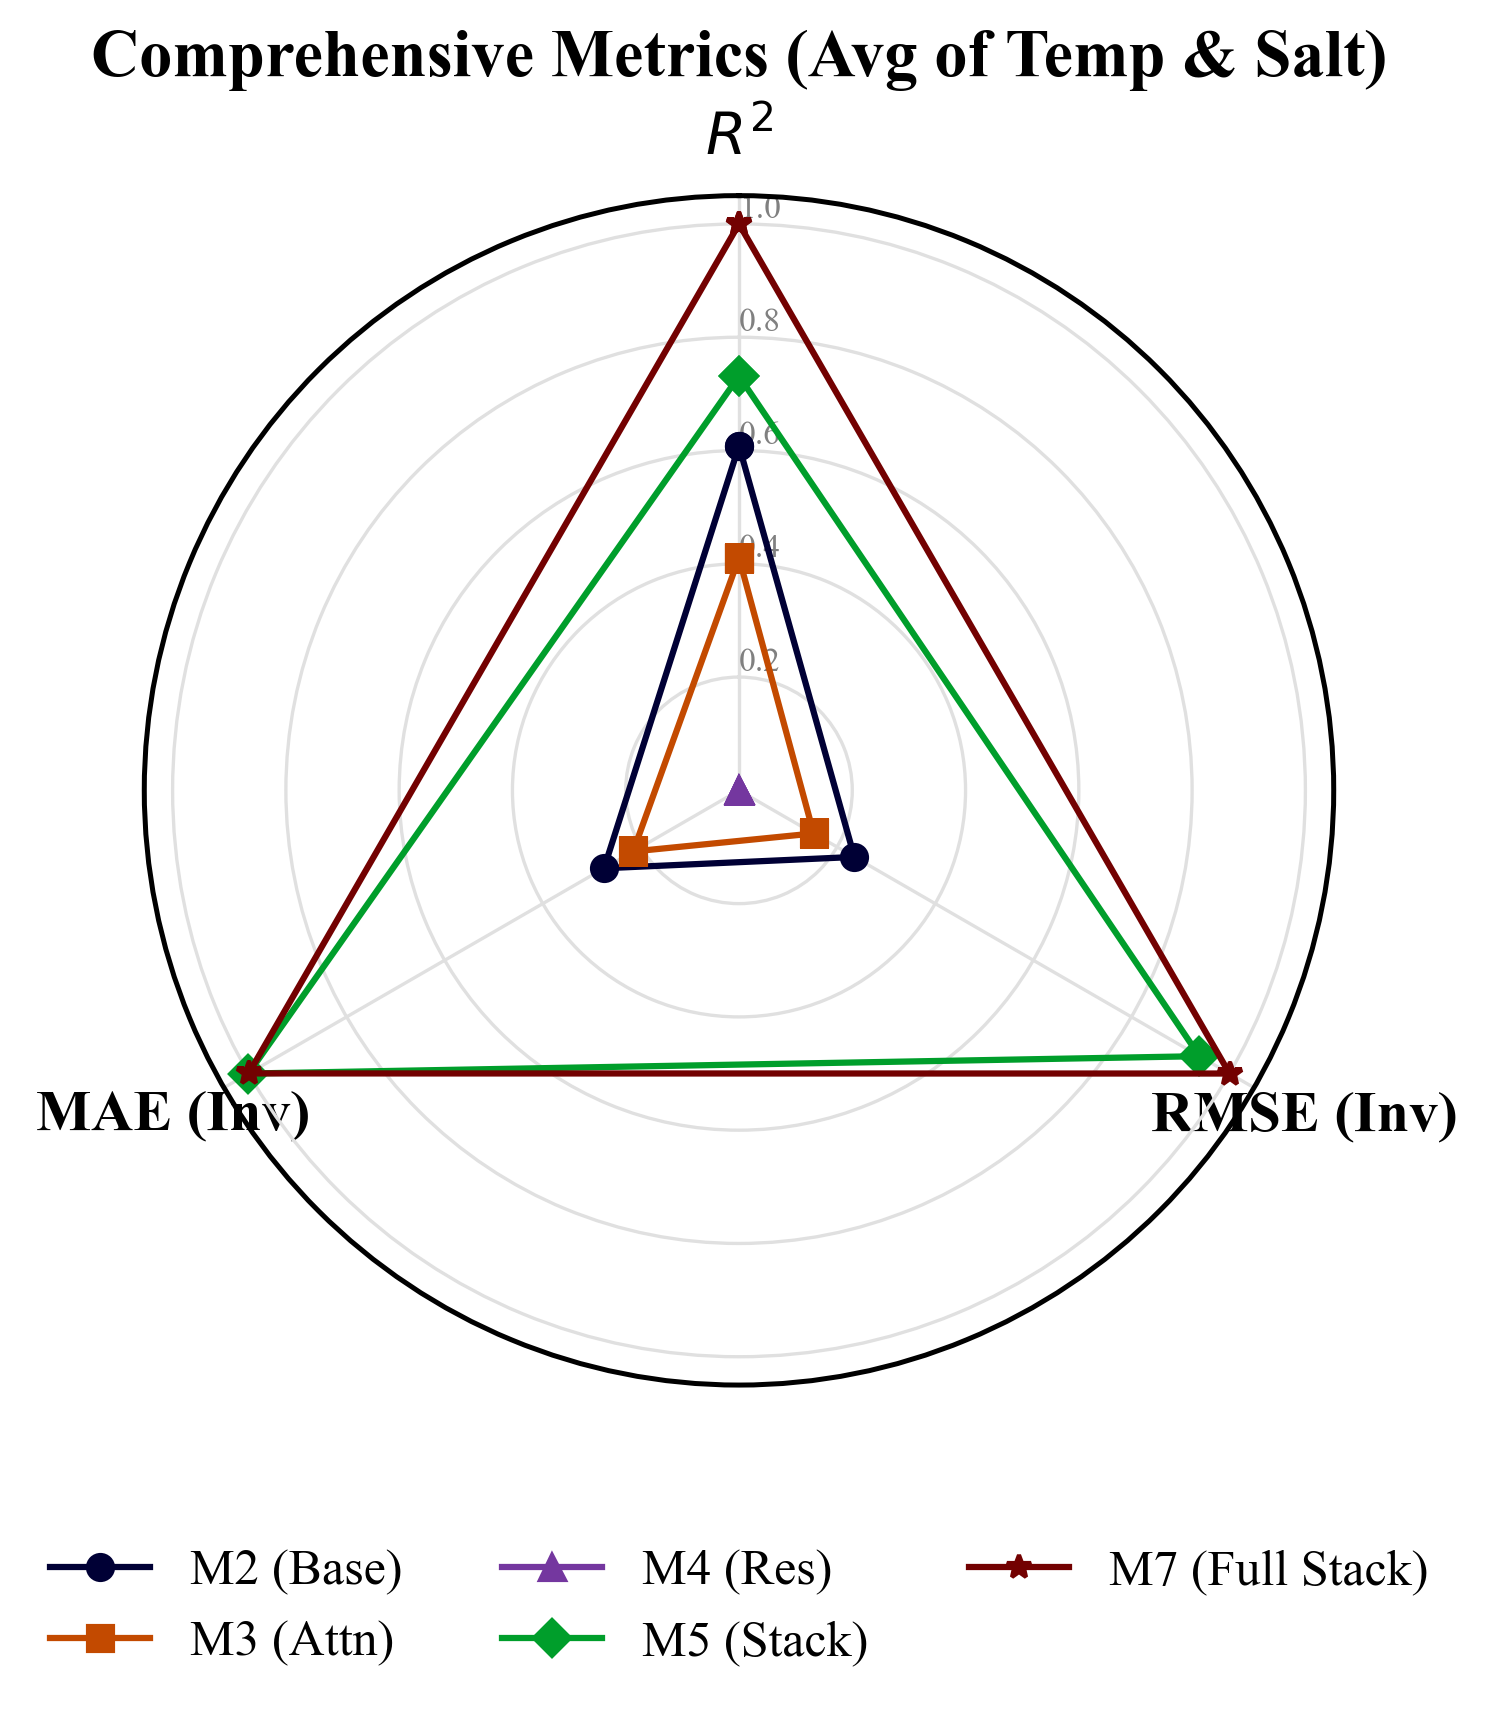
\includegraphics[width=0.48\textwidth]{assets/radar_chart.png}
\caption{Comparison of Core Metrics (R², RMSE, MAE) for Improvement Components}
\label{fig:ablation_radar}
\end{figure}

The metric comparison between Model 1 (Baseline\_CNN) and Model 2 (ConvLSTM\_Base) demonstrates the necessity of introducing ConvLSTM as the backbone model to handle spatiotemporal sequence dependencies. After introducing ConvLSTM, the model's performance on core metrics R², RMSE, and MAE is significantly enhanced, with temperature RMSE reduced by 31.06\% and the overall average improvement rate reaching 19.05\%. This proves the correctness of introducing LSTM time series prediction based on CNN spatial extraction for the ocean temperature and salinity field prediction task in this study.

The comparison group of Model 2 (Base), Model 3 (Attn), Model 4 (Res), and Model 5 (Stack) fully quantifies the improvement effects of the three major improvement measures proposed in this study on the basic ConvLSTM model in the test set. Figure \ref{fig:ablation_r2_line} specifically shows the effect comparison of the R² metric. The introduction of the attention mechanism improved the R² performance of temperature prediction, indicating that it effectively enhanced the model's focus on key areas in temperature prediction. The introduction of the residual connection mechanism improved the temperature prediction R², but deteriorated the effect on salinity. This performance may be related to the data augmentation strategy adopted in this study. Due to the strong latitudinal determinism of temperature and strong regional determinism of salinity, the same-latitude sliding window strategy in this study has physical correlation for temperature, whereas for salinity, the confusing residual signals introduced by data augmentation are further amplified by the residual connection mechanism, causing performance degradation. The introduction of the ARIMA-XGBoost based Stack ensemble (Model 5) reached the optimum in temperature prediction metrics and significantly improved the average salinity prediction metrics by approximately 39.85\% compared to the basic ConvLSTM. The final synthesized model of the three improvement measures (Model 7 (Full + Stacking)) achieved the best effect on salinity and was slightly inferior to Model 5 on temperature, but considering the comprehensive performance of temperature and salinity, combined with Figure \ref{fig:ablation_radar}, this study still considers Model 7 to be the best model.

\begin{figure}[htbp]
\centering
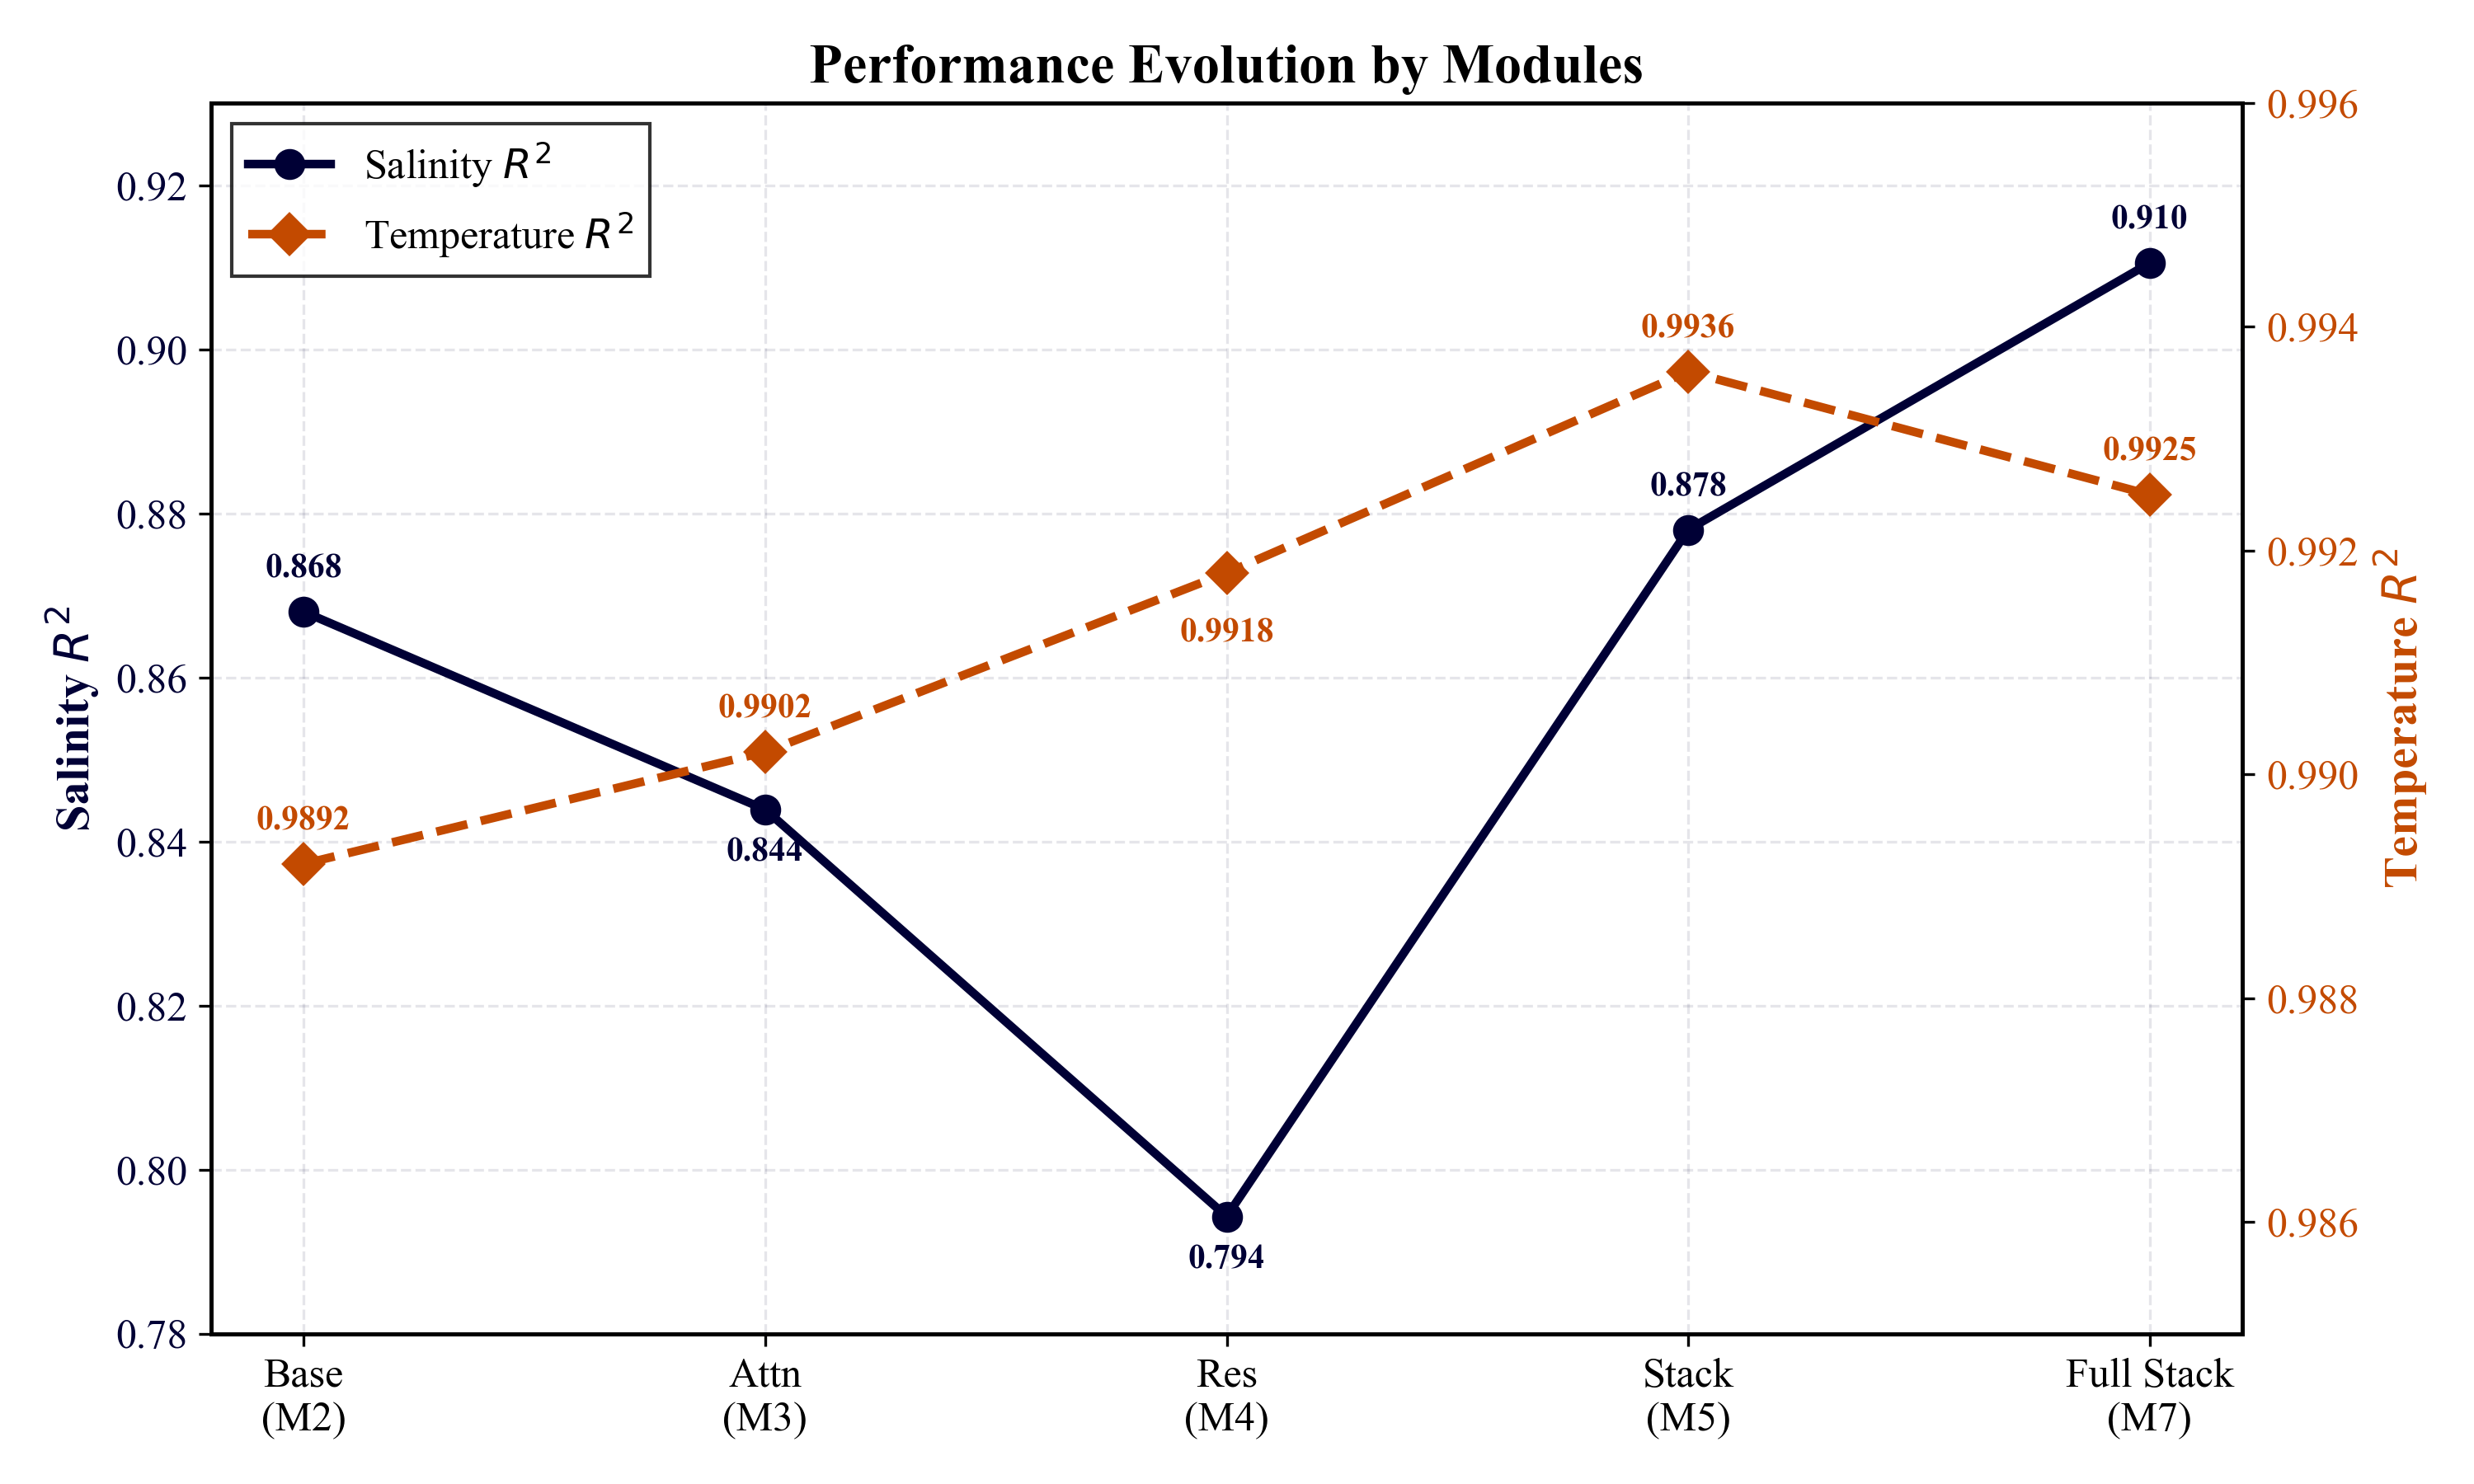
\includegraphics[width=0.48\textwidth]{assets/line_chart_r2-1769754119101-3.png}
\caption{Comparison of R² Metric Improvement for Each Model}
\label{fig:ablation_r2_line}
\end{figure}

Finally, Model 8, Model 9, and Model 10 demonstrate the roles of data augmentation strategies (Model 8 removes equatorial mirror augmentation, Model 9 removes sliding window augmentation) and spatiotemporal encoding (Model 10 removes spatiotemporal encoding). The metrics of Model 8 show that utilizing the physical correlation of temperature equatorial symmetry effectively improved the prediction reliability in terms of temperature. Model 10 reflects the important role of spatiotemporal encoding. Model 9 shows that the data augmentation strategy designed in this paper effectively overcame the problem of short monthly data coverage in the dataset specified in this paper, serving as the foundation for all improvement measures.

\begin{table*}[htbp]
\centering
\caption{Ablation Study Results: R² Score and Improvement Percentage}
\label{tab:ablation_r2}
\resizebox{\textwidth}{!}{%
\begin{tabular}{lcccccccccc}
\toprule
\textbf{Metric} & \textbf{M1 (Base CNN)} & \textbf{M2 (ConvLSTM)} & \textbf{M3 (+Attn)} & \textbf{M4 (+Res)} & \textbf{M5 (+Stack)} & \textbf{M6 (Full)} & \textbf{M7 (Full+Stack)} & \textbf{M8 (NoAug)} & \textbf{M9 (NoSliding)} & \textbf{M10 (NoEnc)} \\ \midrule
\textbf{TEMP R²}        & 0.9773 & 0.9892 & 0.9902 & 0.9918 & 0.9936 & 0.9889 & 0.9925 & 0.9882 & -0.1510 & 0.9870 \\
\textbf{TEMP Improv.(\%)} & 0.00\% & +1.22\% & +1.32\% & +1.48\% & +1.67\% & +1.19\% & +1.55\% & +1.12\% & -115.45\% & +0.99\% \\
\textbf{SALT R²}        & 0.7918 & 0.8680 & 0.8439 & 0.7943 & 0.8780 & 0.8082 & 0.9105 & 0.6872 & 0.2337 & 0.8656 \\
\textbf{SALT Improv.(\%)} & 0.00\% & +9.62\% & +6.58\% & +0.32\% & +10.88\% & +2.07\% & +14.99\% & -13.21\% & -70.48\% & +9.32\% \\ \bottomrule
\end{tabular}%
}

\vspace{1em}

\caption{Ablation Study Results: RMSE and Improvement Percentage}
\label{tab:ablation_rmse}
\resizebox{\textwidth}{!}{%
\begin{tabular}{lcccccccccc}
\toprule
\textbf{Metric} & \textbf{M1 (Base CNN)} & \textbf{M2 (ConvLSTM)} & \textbf{M3 (+Attn)} & \textbf{M4 (+Res)} & \textbf{M5 (+Stack)} & \textbf{M6 (Full)} & \textbf{M7 (Full+Stack)} & \textbf{M8 (NoAug)} & \textbf{M9 (NoSliding)} & \textbf{M10 (NoEnc)} \\ \midrule
\textbf{TEMP RMSE} & 0.1513 & 0.1043 & 0.0996 & 0.0910 & 0.0858 & 0.1057 & 0.0871 & 0.1090 & 1.0773 & 0.1226 \\
\textbf{TEMP Improv.(\%)} & 0.00\% & +31.06\% & +34.17\% & +39.85\% & +43.29\% & +30.14\% & +42.43\% & +27.96\% & -612.20\% & +18.97\% \\
\textbf{SALT RMSE} & 0.4726 & 0.3763 & 0.4093 & 0.4698 & 0.1549 & 0.4537 & 0.1327 & 0.5794 & 0.9068 & 0.1626 \\
\textbf{SALT Improv.(\%)} & 0.00\% & +20.38\% & +13.39\% & +0.59\% & +67.22\% & +4.00\% & +71.92\% & -22.60\% & -91.87\% & +65.59\% \\ \bottomrule
\end{tabular}%
}

\vspace{1em}

\caption{Ablation Study Results: MAE and Improvement Percentage}
\label{tab:ablation_mae}
\resizebox{\textwidth}{!}{%
\begin{tabular}{lcccccccccc}
\toprule
\textbf{Metric} & \textbf{M1 (Base CNN)} & \textbf{M2 (ConvLSTM)} & \textbf{M3 (+Attn)} & \textbf{M4 (+Res)} & \textbf{M5 (+Stack)} & \textbf{M6 (Full)} & \textbf{M7 (Full+Stack)} & \textbf{M8 (NoAug)} & \textbf{M9 (NoSliding)} & \textbf{M10 (NoEnc)} \\ \midrule
\textbf{TEMP MAE} & 0.1162 & 0.0833 & 0.0769 & 0.0765 & 0.0655 & 0.0898 & 0.0705 & 0.0928 & 0.7988 & 0.0846 \\
\textbf{TEMP Improv.(\%)} & 0.00\% & +28.31\% & +33.82\% & +34.14\% & +43.63\% & +22.72\% & +39.33\% & +20.14\% & -587.44\% & +27.19\% \\
\textbf{SALT MAE} & 0.3533 & 0.2695 & 0.2905 & 0.3440 & 0.1090 & 0.3524 & 0.1041 & 0.4502 & 0.7283 & 0.1155 \\
\textbf{SALT Improv.(\%)} & 0.00\% & +23.72\% & +17.77\% & +2.63\% & +69.15\% & +0.26\% & +70.53\% & -27.43\% & -106.14\% & +67.31\% \\ \bottomrule
\end{tabular}%
}
\end{table*}

\section{Conclusion and Future Work}

\subsection{Main Conclusions}

This paper proposes a spatiotemporal sequence prediction framework based on ConvLSTM, integrating attention mechanism, residual refinement module, and ARIMA-Stacking error correction strategy, for multi-step prediction of subsurface temperature and salinity in the Western Pacific. Extensive experiments on multi-source ocean data such as Argo, AVISO, and CCMP show that the proposed method is significantly superior to CNN and ConvLSTM benchmark models in terms of prediction accuracy, spatiotemporal structure preservation capability, and physical consistency, demonstrating excellent prediction performance and application potential. The main conclusions are as follows:

\begin{enumerate}
\renewcommand{\labelenumi}{\alph{enumi})}
\item The proposed model shows significant advantages in multi-step prediction tasks of temperature and salinity, especially in salinity, a high-noise and difficult-to-predict variable. After introducing the ARIMA-Stacking heterogeneous ensemble strategy, the salinity prediction error dropped significantly, effectively alleviating the modeling difficulties of strong salinity signal noise and drastic variation.

\item Visualization analysis shows that the model has almost no obvious phase lag and morphological distortion in the multi-step recursion process, and the vertical profile structure is maintained well.

\item By introducing Potential Density and Spiciness as physical consistency evaluation indicators, it is verified that the model maintains the nonlinear coupling relationship between temperature and salinity well, and the prediction results show higher credibility in derived physical quantities.

\item Ablation experiments systematically verified the effectiveness of attention mechanism, residual refinement module, spatiotemporal positional encoding, data augmentation, and Stacking ensemble strategy. Each component synergizes with each other to jointly improve the overall performance and generalization ability of the model.
\end{enumerate}

\subsection{Limitations and Future Work}

Although the method proposed in this paper has achieved good results in the temperature and salinity prediction task in the Western Pacific, there are still the following deficiencies, which need to be further improved in subsequent research:

\begin{enumerate}
\renewcommand{\labelenumi}{\alph{enumi})}
\item The current model is mainly designed for short-to-medium-term (months) prediction. As the forecast lead time extends, the phenomenon of error accumulation gradually appears, and the long-term sequence prediction ability still needs to be strengthened.

\item The abnormal ocean response under strong external forcing such as typhoons and extreme El Niño has not been systematically evaluated, and the robustness of the model in extreme event scenarios still needs to be verified.

\item To address the issue of insufficient temporal data in the dataset for training, the data augmentation strategy designed in this paper expands the training data from the physical spatial perspective, utilizing the strong latitudinal correlation of temperature, while ignoring the weak correlation between salinity and latitude.
\end{enumerate}

Correspondingly, future research can suppress deepened from the following directions:

\begin{enumerate}
\renewcommand{\labelenumi}{\alph{enumi})}
\item Introduce differentiable physical constraints (such as primitive equation residuals, conservation laws, etc.) to construct physics-informed neural networks to further enhance the physical consistency and long-term stability of prediction results.

\item Extend to fully three-dimensional spatiotemporal modeling architecture (such as 3D ConvLSTM, 3D Transformer, or 4D variational neural networks) to achieve simultaneous synchronous prediction from surface to deep layers, and more completely capture vertical mixing and baroclinic processes.

\item Combine Graph Neural Networks (GNN) to handle unstructured grids or irregular boundaries, improving the model's adaptability to complex coastal topography and high-resolution non-uniform grids.

\item Explore model compression, knowledge distillation, and efficient ensemble methods to reduce computational overhead while maintaining prediction accuracy, promoting the deployment of models to real-time business and on-board processing scenarios.

\item Design data augmentation strategies specifically for salinity that have strong physical correlations with it.
\end{enumerate}

In summary, the deep spatiotemporal-statistical fusion prediction framework proposed in this paper provides an effective technical path for high-precision subsurface ocean temperature and salinity forecasting. In the future, through deeper integration of physical constraints and upgrading of 3D modeling technology, it is expected to further improve the long-term predictability of ocean environmental elements.

\section*{Data Availability Statement}
The data supporting the conclusions of this study can be directly obtained from the following public repositories:
\begin{enumerate}
    \renewcommand{\labelenumi}{\alph{enumi})}
    \item In-situ derived Argo temperature and salinity profiles and their climatology data: Asia-Pacific Data-Research Center (APDRC, \url{http://apdrc.soest.hawaii.edu/projects/Argo/data/gridded/On_standard_levels/index-1.html}), selected time span: 2005—2020.
    \item Sea Surface Height (SSH) data: AVISO satellite altimeter data (\url{http://www.aviso.altimetry.fr}), selected time span: 1993—2020.
    \item Sea Surface Wind (SSW) data: CCMP wind analysis data (\url{https://rda.ucar.edu/datasets/ds745.1/}), selected time span: 1987—2020.
\end{enumerate}

\section*{Funding}
This research was supported by Key Laboratory of Southeast Coast Marine Information Intelligent Perception and Application, MNR, NO.24205 and XMU Training Program of Innovation and Enterpre-neurship for Undergraduates (S202510384570).

\section*{Acknowledgments}

We thank the Global Argo Float Program (www.argo.ucsd.edu) and Copernicus Marine Environment Monitoring Service (CMEMS, marine.copernicus.eu) for providing high-quality temperature, salinity, and sea surface dynamic environment data.

We thank all colleagues in the laboratory for their beneficial discussions and selfless help during the research process. We thank the anonymous reviewers and journal editors for their valuable revision suggestions, which greatly improved the quality of this paper.

We acknowledge the use of AI tools for language polishing, formatting, and translation work.

Finally, we would like to express our sincerest gratitude to our mentors, friends, and family for their continuous support and encouragement during the research and writing process.

%zotero导入
\bibliographystyle{unsrt}
\bibliography{ref}

\end{document}
